\chapter{Results and Applications Involving 1D Estimation}
\label{chap:results}

This chapter showcases results generated using the \ac{1D} estimation
technique outlined in the previous chapter. Furthermore, two means by
which the \ac{1D} estimation procedure can be harnessed as part of
specific applications are presented.
\Cref{sec:evaluation} provides some examples of how the estimation
routine performs on \ac{1D} \ac{NMR} datasets acquired using a standard
pulse-acquire experiment. \Cref{sec:seq} illustrates how the basic \ac{1D}
estimation routine
can be extended to enable the consideration of datasets comprising a series of
\acp{FID} which feature attenuations in signal amplitudes across increments,
including inversion recovery and diffusion experiments. Finally,
\cref{sec:bbqchili} describes a protocol to generate ultra-broadband spectra
through application of a single \ang{90} \acl{FS} pulse, which are devoid of
quadratic phase dependencies as well as baseline distortions.

All the results presented were produced on the same computer (see
\cref{rem:workstation}), using the \ac{EsPy} package which is
described in \cref{chap:nmrespy}. Details about the datasets generated are
provided in \cref{chap:datasets}.

\section{Conventional \ac{1D} Datasets}
\label{sec:evaluation}

As mentioned in \cref{subsec:phase-variance}, one of the disadvantages of
\ac{SVD}-based methods like the \ac{MPM} is their propensity to generate
parameter estimates featuring oscillators with spurious phase behaviour. Such
behaviour is most prevalent in \acp{FID} which (a) feature signals with very
similar frequencies and (b) that have a low \ac{SNR}.
To assess the effectiveness of including the phase variance-regularised
\ac{NLP} routine, comparisons are now made with results generated with the
\ac{MPM} in isolation.

For the experimental datasets considered (\cref{subsec:andro,subsec:cyclo}),
the data was pre-processed using \textsc{Bruker}'s \textsc{TopSpin} software,
using the series of commands \texttt{ft; pk; abs}; these perform \ac{FT},
automatic phase correction, and baseline correction, respectively. The data was
then converted back to the time-domain using \ac{IFT} prior to filtering and
estimation.

\subsection{``Twenty Signals''}
%%% Previously had this as landscape:
% \begin{sidewaysfigure}
%     \centering
%     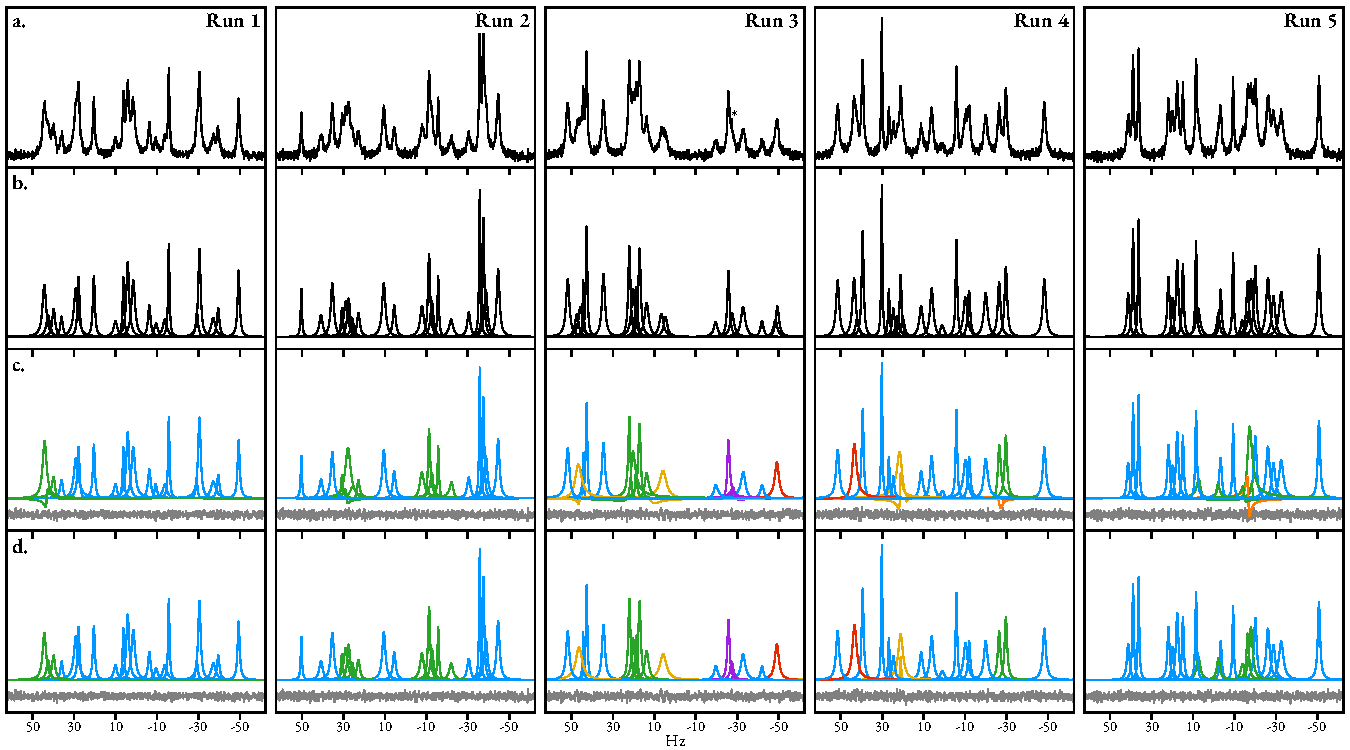
\includegraphics{mpm_vs_nlp/mpm_vs_nlp_landscape.pdf}
%     \caption[
%         The result of estimating a series of 5 simulated \acsp{FID}
%         using both the \acs{MPM} in isolation, and also with phase
%         variance-regularised \acs{NLP} used afterwards.
%     ]{
%         The result of estimating a series of 5 simulated \acp{FID} comprising
%         20 signals. See the main text for details on how the \acp{FID} were
%         constructed.
%         \textbf{a.} Spectra of the \acp{FID} generated.
%         \textbf{b.} Spectral lines corresponding to the set of signals
%         used to generate each \ac{FID}.
%         \textbf{c.} Plots of peaks for each oscillator generated using
%         the \acs{MPM}.
%         \textbf{d.} An equivalent plot for the result after applying phase
%         variance-regularised \acs{NLP}, using the \acs{MPM} result as an
%         initial guess.  Also included in c and d are the
%         residual between the data and the estimated model (grey
%         line). The colouring of the oscillators in c and d is described
%         in the main text.
%     }
%     \label{fig:mpm_vs_nlp}
% \end{sidewaysfigure}
\begin{figure}
    \centering
    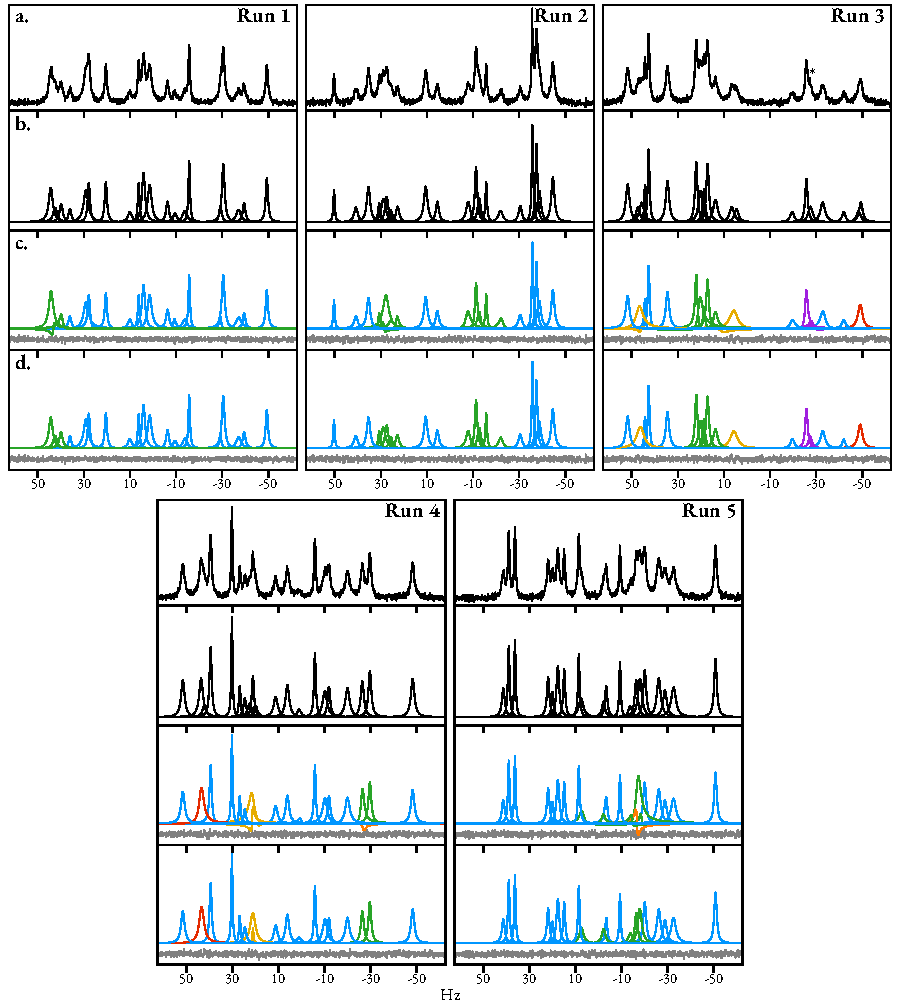
\includegraphics{mpm_vs_nlp/mpm_vs_nlp_portrait.pdf}
    \caption[
        The result of estimating a series of 5 simulated \acsp{FID}
        using both the \acs{MPM} in isolation, and also with phase
        variance-regularised \acs{NLP} used afterwards.
    ]{
        The result of estimating a series of 5 simulated \acp{FID} comprising
        20 signals. See the main text for details on how the \acp{FID} were
        constructed.
        \textbf{a.} Spectra of the \acp{FID} generated.
        \textbf{b.} Spectral lines corresponding to the set of signals
        used to generate each \ac{FID}.
        \textbf{c.} Plots of peaks for each oscillator generated using
        the \acs{MPM}.
        \textbf{d.} An equivalent plot for the result after applying phase
        variance-regularised \acs{NLP}, using the \acs{MPM} result as an
        initial guess.  Also included in c and d are the
        residual between the data and the estimated model (grey
        line).
        \correction{
            Blue oscillators are those produced by the MPM which closely agree
            with a true signal.  Green oscillators are affected notably by the
            NLP routine, and end up in good agreement with a true signal.
            Orange oscillators were excessive oscillators generated by the MPM,
            which were removed during the NLP routine, leading to a
            parsimonious fit of the remaining (green) oscillators in the
            frequency neighbourhood.  Yellow oscillators denote cases where the
            number of oscillators produced by the MPM matched the number of
            true signals in a given frequency neighbourhood. However one of the
            oscillators was removed during the NLP routine, leading to an
            under-fit of the neighbourhood.  Red oscillators denote an
            under-fit of a frequency neighbourhood by the MPM.  Purple
            oscillators denote an over-fit of a frequency neighbourhood by the
            MPM, with none of the oscillators being removed during NLP
            (\textit{cf.} orange oscillators which are removed during NLP).
        }
    }
    \label{fig:mpm_vs_nlp}
\end{figure}
A series of five simulated \acp{FID} were constructed using
\cref{eq:hypercomplex-fid} with $D=1$. For each \ac{FID}, a model order
of $M=20$ was used, the number of points sampled was $N = 1024$, the sweep
width was $\fsw=\qty{125}{\hertz}$, and the transmitter offset was $\foff
= \qty{0}{\hertz}$.  Each oscillator was assigned a phase of \ang{0}, while the
amplitudes, frequencies and damping factors were drawn at random from the
following distributions
$\forall m \in \lbrace 1, \cdots, 20\rbrace$:
$a_m \sim \mathcal{U}(1, 5)$, $f_m \sim \mathcal{U}(\qty{-55}{\hertz},
\qty{55}{\hertz})$, $\eta_m \sim \mathcal{U}(\qty{2}{\per\second},
\qty{8}{\per\second})$. The frequencies were subjected to an additional
constraint; no two signals were permitted to have frequencies that
differed by less than $\nicefrac{4 \fsw}{N} \approx \qty{0.49}{\hertz}$.
Each noiseless \ac{FID} $\bx$ was then corrupted with \ac{AWGN}, with a target
\ac{SNR} of \qty{25}{\deci\bel}, such that the desired noise variance for each
\ac{FID} was given by (\emph{cf.} \cref{eq:snr,eq:snr-db}):
\begin{equation}
    \sigma^2 = \frac{1}{20^{2.5} \times 1024}
        \sum_{n=0}^{1023} \lvert x_n \rvert^2.
\end{equation}
The spectra of the simulated \acp{FID} are presented in
\cref{fig:mpm_vs_nlp}.a, with the set of oscillator peaks which contribute
to the spectrum in \cref{fig:mpm_vs_nlp}.b. With the criteria used to
constructed the datasets, it can be seen they feature signals which often
suffer from severe overlap, with the high noise variance compounding the
opportunity to clearly identify all contributing signals.

For each \ac{FID}, the \ac{MPM} was performed, assuming a model order of
30, constituting a considerable over-fit of oscillators. The \ac{MDL} tended to
produce under-estimates of $M$ when applied to these \acp{FID}, so the
hard-coded value was used instead to ensure sufficient oscillators were given
to the model. The under-estimates were likely due to the
high \ac{SNR} of the signals\,---\,recall the red signal in \cref{fig:mdl}\,---\,in
conjunction with severe signal overlap. When an excessive model order is
provided to the \ac{MPM}, it is typical that oscillators corresponding to the
noise subspace of the data matrix $\Hy$ are characterised by small amplitudes
and/or very small damping factors. For this reason, prior to subjecting the
\ac{MPM} result to \ac{NLP}, oscillators which satisfied $a_m < 0.1$ and/or
$\eta_m < \qty{0.7}{\per\second}$ were removed from the parameter set. The
individual oscillators which make up the \ac{MPM} result after purging spurious
components are displayed in \cref{fig:mpm_vs_nlp}.c, along with the
residual between the data and the estimated model (i.e. the sum of all
oscillator peaks).

The \ac{MPM} consistently generated models which agreed well with the data
in a least squares sense, as as evidenced by the residuals in
\cref{fig:mpm_vs_nlp}.c.
However, it can be seen that in several spectral regions across the datasets,
especially ones that are highly crowded, oscillators possess parameters which
deviate significantly from the true signal parameters used to constructed the
\acp{FID}.
Most notably, individual oscillator phases regularly stray far from \ang{0},
and their associated amplitudes are often considerably different too.
In \cref{fig:mpm_vs_nlp}.c, blue oscillators are those which
are in very close agreement with a particular true signal in the data.
Oscillators with other colours are not in agreement with a true signal,
with the different colourings described shortly.
The desired outcome of the \ac{NLP} routine is for it to adjust the
parameters associated with non-blue oscillators in \cref{fig:mpm_vs_nlp}.c such
that they agree with true signals, while having little to no effect on those of
the blue oscillators. The results after application of \ac{NLP} are provided in
\cref{fig:mpm_vs_nlp}.d.

In discussing the outcome of the routine, it will be helpful to employ the
concept of a \emph{frequency neighbourhood}, a loose term which describes a
small, continuous subset of frequencies within the spectral window. As the
\ac{NLP} routine involves taking small steps
in parameter space over a number of iterations, it is unlikely that an
oscillator which starts off with a frequency far away from a particular
frequency neighbourhood will eventually enter it. As such, in order for the
\ac{NLP} routine to successfully estimate the signals within a given frequency
neighbourhood of the data, sufficient model oscillators need to present within
the neighbourhood in the initial guess.

Cases where the
\ac{MPM} generated enough oscillators for a given frequency neighbourhood,
albeit with parameters which noticeably deviate from the true signals are
coloured either green or yellow. Green oscillators are those which the \ac{NLP} routine
was able to adjust so as to to achieve agreement with true signals;
they indicate improvements to the estimation result in comparison with the \ac{MPM}
in isolation. Conversely, yellow oscillators denote cases where, though
sufficient oscillators existed in the frequency neighbourhood in the initial
guess, the \ac{NLP} routine evolved such that at least one of the oscillators
was driven by the phase variance constraint to acquire a negative amplitude,
leading to it being removed from the parameter set. This typically occurred with
oscillators that had an initial phase which was either $>
\nicefrac{\pi}{2}$\,\unit{\radian}, or $< -\nicefrac{\pi}{2}$\,\unit{\radian}.
Therefore, yellow oscillators indicate cases where the final result
under-fit the dataset.

There are a couple of instances, denoted by red oscillators,
where the \ac{MPM} assigned too few oscillators to a particular frequency
neighbourhood, and as such the \ac{NLP} routine would not have been able to
yield any major improvement. This occurred in what can safely be described as
fiendishly difficult cases, where severe signal overlap and low \ac{SNR} make
it very difficult to associate certain spectral regions with more than one
signal by eye.

The final two oscillator groupings, coloured purple and orange respectively,
indicate scenarios where the \ac{MPM} generated more oscillators than true
signals in a given frequency neighbourhood (i.e. the data was over-fit in these
regions). Orange
oscillators we purged by the \ac{NLP} routine as they acquired negative
amplitudes. This enabled parsimonious fits of the relevant frequency neighbourhoods by
the oscillators which remained, i.e. the green oscillators in close proximity
to the orange ones in \cref{fig:mpm_vs_nlp}.c. Finally, the purple oscillators
denote the one
occasion (Run 3) where an over-fit occurred, and the model order was not
successfully reduced by the \ac{NLP} routine. One of the purple oscillators in
the \ac{MPM} appears to agree closely with a significant ``blip'' in the noise,
denoted by an asterisk in \cref{fig:mpm_vs_nlp}.a.
The over-fit has therefore occurred because this noise component was
incorporated into the final result; it was neither purged based on the
amplitude and damping factor criteria outlined above, nor by acquiring a
negative amplitude during \ac{NLP}.

\subsection{Andrographolide}
\label{subsec:andro}
\begin{figure}
    \centering
    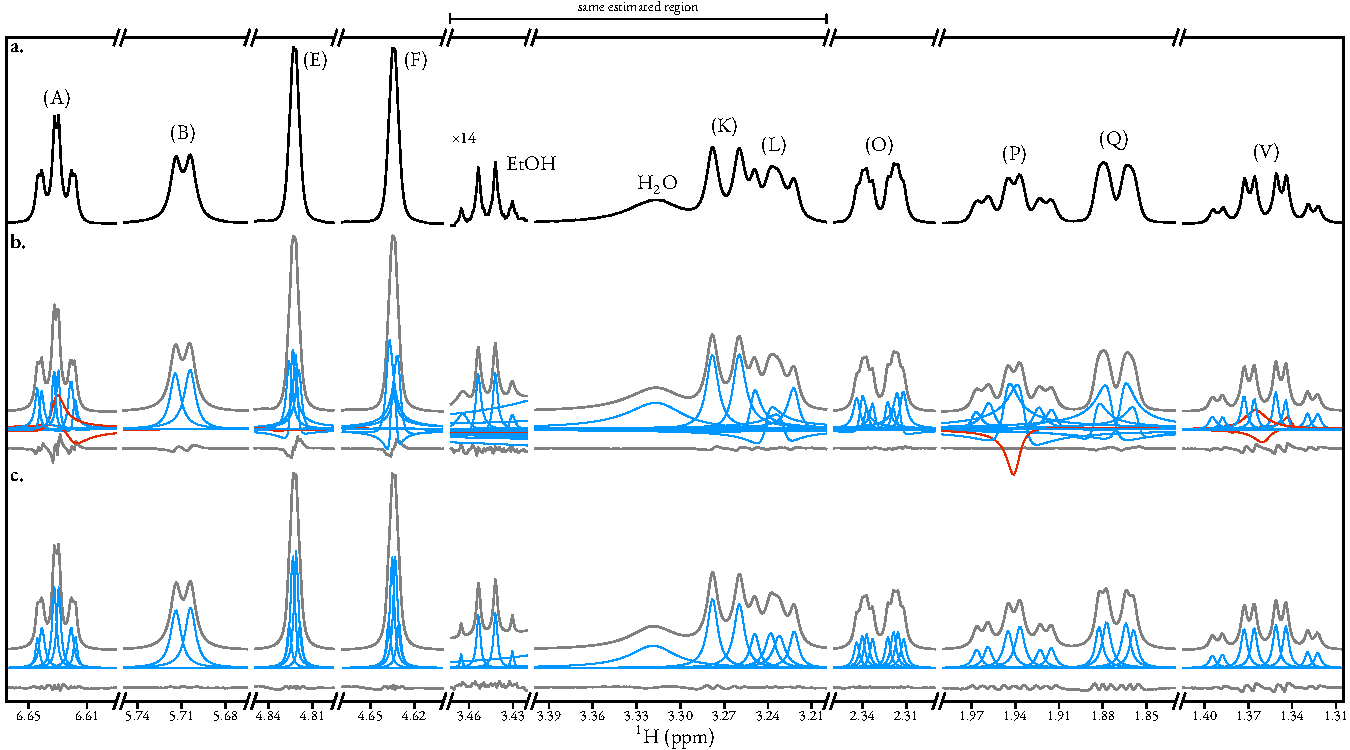
\includegraphics{andrographolide_onedim/andrographolide_onedim.pdf}
    \caption[
        The result of applying the estimation routine to selected regions of a
        pulse-acquire dataset of andrographolide.
    ]{
        The result of applying the estimation routine to selected regions of a
        pulse-acquire dataset of andrographolide in \acs{DMSOd6}.
        \textbf{a.} The structure of andrographolide.
        \textbf{b.} Spectral regions considered.
        \textbf{c.} The result of applying the \acs{MPM} to the regions, with
        the model order predicted using the \acs{MDL}. Blue and red lines denote
        individual oscillator peaks, while the grey line above is the sum of all
        oscillators. They grey line below is the residual between the data and
        the model.
        \textbf{d.} The result after convergence of the \acs{NLP} routine, again
        with the model above and residual below.
        Red peaks in b correspond to oscillators which acquire negative
        amplitudes and are removed during the \acs{NLP} routine.
        One of the estimated regions has been split in two in the
        figure to save space, with one half, featuring a signal from ethanol,
        being magnified.
    }
    \label{fig:andro-onedim}
\end{figure}
\Cref{fig:andro-onedim} illustrates the outcome of applying the
estimation routine to a \textsuperscript{1}H dataset of
andrographolide (\cref{fig:structures}.a) in \acs{DMSOd6}, acquired with
a \qty{600}{\mega\hertz} spectrometer.
Various spectral regions were chosen for study, and for each one, a
frequency-filtered sub-\ac{FID} was produced using the approach in
\cref{sec:filtering}.
The \ac{MPM} was used to generate an initial guess of parameters, using the
\ac{MDL} to predict the model order in each case. The result of applying the
\ac{MPM} are presented in \cref{fig:andro-onedim}.b. The initial guess
was then subjected to \ac{NLP}, giving rise to the result
\cref{fig:andro-onedim}.c.

The \ac{NLP} routine was effective at resolving the spurious phase behaviour
often generated by the \ac{MPM}.
The estimation method's ability to parametrise signals with high
dynamic range and high variation of damping factors is also evidenced;
a broad intense singlet from water, and a low-intensity quartet from
residual ethanol in the sample, present in the same sub-\ac{FID}, could both
estimated admirably for example.
For some of the sub-\acp{FID} considered, the \ac{MPM} output featured
oscillators, commonly with very high damping factor and/or phases far from
\ang{0}, which were removed during the \ac{NLP} routine (see the red
peaks in panel b). The removal of these, along with the enforcement
of consistent oscillator phases, leads to parameter
estimates which describe the apparent multiplet structures associated with each
spin well. \Cref{tab:andro-multiplets} provides an overview of the
most significant couplings associated with the spins giving rise to the
multiplet structures considered.
\begin{table}
\centering
\begin{tabular}{c c c}
\hline
Spin  & Coupling partners & Multiplet structure \\
\hline
\multicolumn{3}{c}{\textbf{Andrographolide}}\\
\hline
(A) & (D)\textsuperscript{long}, (M)\textsuperscript{vic}, (N)\textsuperscript{vic} & ddd (\emph{dt}) \\
(B) & (D)\textsuperscript{ex} & d \\
(E) & (F)\textsuperscript{vinyl} \dots & d\dots \\
(F) & (E)\textsuperscript{vinyl} \dots & d\dots \\
(K) & (J)\textsuperscript{gem}, (H)\textsuperscript{ex} & d \\
(L) & (C)\textsuperscript{ex}, (T)\textsuperscript{180}, (U)\textsuperscript{60} & dd \\
(O) & (P)\textsuperscript{gem}, (R)\textsuperscript{60}, (V)\textsuperscript{60} & ddd \\
(P) & (O)\textsuperscript{gem}, (R)\textsuperscript{60}, (V)\textsuperscript{180} & ddd (\emph{dt}) \\
(Q) & (M)\textsuperscript{vic}, (N)\textsuperscript{vic} \dots & dd\dots \\
(V) & (O)\textsuperscript{60}, (P)\textsuperscript{180}, (R)\textsuperscript{g}, (W)\textsuperscript{180} & dddd (\emph{dq}) \\
\hline
\multicolumn{3}{c}{\textbf{Cyclosporin A}}\\
\hline
(A) & diastereotopic pair on \textsuperscript{\textbeta}C & dd \\
(B) & ---''--- & dd \\
(C) & ---''--- \& amide proton & ddd (\emph{dt}) \\
(D) & proton on \textsuperscript{\textbeta}C \& amide proton & dd \\
(E) & methyl protons on \textsuperscript{\textbeta}C \& amide proton & dq \\
(F) & ---''--- & dq (\emph{quintet}) \\
\hline
\end{tabular}
\caption[
    The major coupling partners associated with spins in andrographolide and
    cyclosporin A, along with the multiplet structures that arise.
]{
    The major coupling partners associated with spins in andrographolide and
    cyclosporin, considered in \cref{fig:andro-onedim,fig:cyclosporin}
    respectively, along with the multiplet structures that arise.
    For andrographolide, coupling partners are labelled as follows:
    \textsuperscript{vinyl} geminal coupling between two vinylic protons,
    \textsuperscript{ex} geminal coupling between two protons, with one
    bonded to an oxygen, leading to exchange decoupling\cite[Section
    2.6.1.5]{Claridge2016},
    \textsuperscript{gem} geminal coupling between two spins whose dihedral
    angle is not fixed,
    \textsuperscript{long} long-range coupling,
    \textsuperscript{vic} vicinal coupling,
    \textsuperscript{60} geminal coupling, with a fixed dihedral angle of
    \ang{60} between the spins,
    \textsuperscript{180} geminal coupling, with a fixed dihedral angle of
    \ang{180} between the spins.
    All cyclosporin couplings for the spins considered are geminal couplings.
    In cases where the observed multiplet structure is different to the true
    structure, the observed structure is is in brackets. Ellipses denote cases
    where more (long-range) coupling partners are likely, based on the
    estimation result generated/the appearance of the spectrum, though these
    have not been explicitly assigned.
}
\label{tab:andro-multiplets}
\end{table}

One of the most challenging aspects of estimating \ac{NMR} signals is
the common presence of signals within the dataset that have incredibly similar
frequencies due to the influence of scalar couplings.
Molecules with fused ring systems such as andrographolide are prime examples of spin
systems which generate such datasets, as they tend to have very dense coupling
networks leading to complex multiplet structures. Furthermore, fused systems often
exhibit appreciable long-range couplings (between spins separated by four or
more bonds) alongside ubiquitous two-bond (\emph{geminal}) and three-bond
(\emph{vicinal}) couplings. Long range couplings can be particularly challenging to
resolve, as they are often of a comparable magnitude to the spectral resolution
($\nicefrac{\fsw}{N}$), making individual signals barely perceptible.

Take the multiplet structure from spin (Q) as an example of a particularly
challenging estimation problem.
(Q) has separate vicinal couplings to the
diastereotopic protons (M) and (N); these are the couplings to
(Q) of greatest magnitude. If these were the only couplings, a doublet of doublets
(dd) structure would be expected, which is what has been generated by
the estimation routine.
However, a comparison of the data and
the model indicates that there is a clear discrepancy between the two,
evidenced by systematic deviations in the residual; this feature hints at an
under-fit of the data.
% The \ac{MPM} generated oscillators with phases deviating far from \ang{0},
% which enabled good agreement with the data in a residual sense, though of
% course such a set of oscillators is unrealistic in the context of a phased
% \ac{FID}.
Long-range couplings with magnitudes that are large enough to influence the
appearance of (Q)'s multiplet structure are likely to be present, which leads
to frequency neighbourhood in which all contributing signals are too poorly
resolved to realistically gleam any further meaningful information, at least at
the field strength used.

As a second illustration, the multiplet structure corresponding to spin (V) is also
under-fit, this time because the presence of a number of couplings of similar
magnitude leads to resonances coalescing at roughly the same frequency. A
multiplet structure featuring 16 resonances forming in ``dddd'' structure is
expected. However, 3 of the couplings are of similar magnitudes, such that
many of the contributing signals coalesce to form what is apparently a quartet
of doublets (dq).
The estimation routine was able to resolve this dq structure,
however the large deviations in the residual again imply that under-fitting has
occurred, and each oscillator in the parameter set is in fact being used to fit
two or more signals present in the \ac{FID}. Again, at the field strength used
to acquire the \ac{FID}, it is unlikely that an accurate resolution of all 16
signals by estimation is feasible.

% At this point, with two examples provided of cases where poor \ac{RSS} fits
% have resulted, one may question whether the underlying model is actually suited
% to describe the data.
% There is for example precedent for fitting oscillators with non-exponential
% decay profiles\,---\,profiles which lead to Voigt and Gaussian spectral
% lineshapes are common\,---\,to improve the model fit\cite{Sima2007}.
% However, for some multiplet structures in Figure \ref{fig:andro-onedim},
% exceptionally good agreement between the model and data are made, using a
% parsimonious set of parameters.
With three couplings of different magnitude, spin (O) exhibits a ``ddd''
multiplet structure in which all 8 signals are discernible. The \ac{NLP}
routine performed well in taking the initial guess from the
\ac{MPM}\,---\,featuring the correct number of oscillators albeit with
spurious phases\,---\, and generating a well-phased set of oscillators defining
the ddd structure, with a very small associated residual. This highlights that
in cases where all signals present in a given frequency neighbourhood are
resolvable, effective estimation results are achievable.

\subsection{Cyclosporin A}
\label{subsec:cyclo}
\begin{figure}
    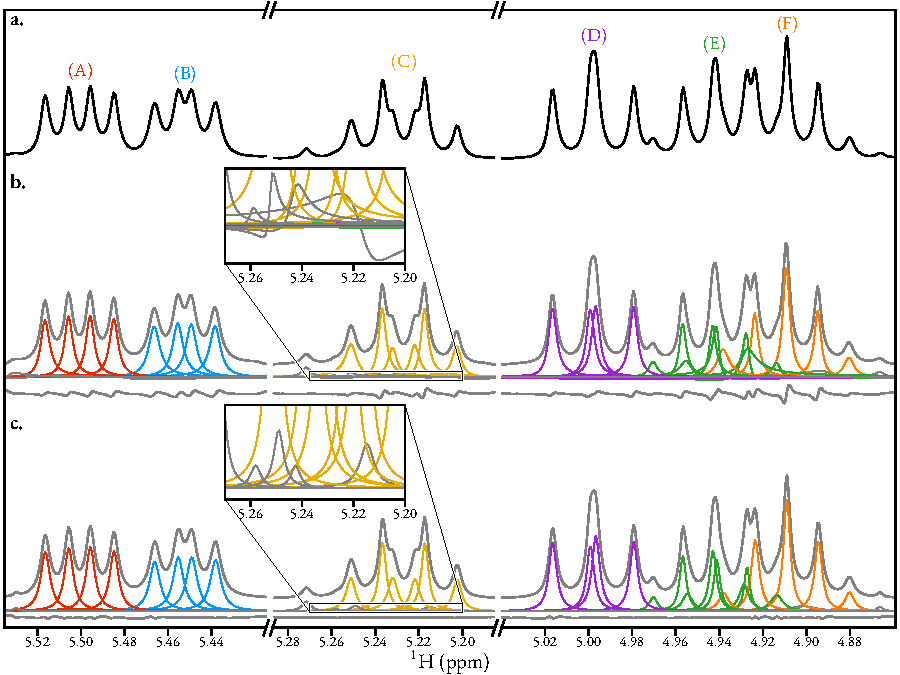
\includegraphics{cyclosporin/cyclosporin.pdf}
    \caption[
        The result of applying the estimation routine to selected regions of a
        pulse-acquire dataset of cyclosporin A.
    ]{
        The result of applying the estimation routine to selected regions of a
        pulse-acquire dataset of cyclosporin A in benzene-d\textsubscript{6}.
        \textbf{a.} The structure of cyclosporin A, with relevant proton
        environments highlighted.
        \textbf{b.} Spectral regions considered.
        \textbf{c.} The result of applying the \acs{MPM} on the regions, with
        the model order predicted using the \acs{MDL}.
        The grey lines above and below the individual oscillator peaks denote
        the sum of all oscillators and the residual between the data and the
        model, respectively.
        \textbf{d.} The result after convergence of the \acs{NLP} routine,
        presented in the same format as panel c.
        Coloured oscillators have been mapped to particular cyclosporin A
        environments. Grey oscillators are not associated with
        cyclosporin A; these are likely due to impurities in the sample.
    }
    \label{fig:cyclosporin}
\end{figure}
The estimation routine was also applied to selected regions of a
\proton\ pulse-acquire dataset of cyclosporin A
(\cref{fig:structures}.b), a cyclic peptide comprising 11 amino
acids, in benzene-d\textsubscript{6}.
The regions considered all comprise
signals arising from protons bound to C\textsuperscript{\textalpha} atoms in
the peptide backbone\cite{Verma2018}.
The estimation procedure used was equivalent to
that used for the andrographolide example.

For the most downfield region
considered, featuring signals from spins (A) and (B), the \ac{MPM} performed
admirably, with the two well-resolved dd multiplet structures present
accurately parametrised by the 8 oscillators in the model; the \ac{NLP} routine
hardly perturbed the initial guess as a result.

In the middle region, which features a doublet of triplets (dt) multiplet structure
from spin (C), low intensity ``shoulders'' are noticeable;
these are likely from low-concentration impurities in the sample. The \ac{MPM}
was able to resolve the dt structure, and characterise
some low intensity signals too, though the phases of these are highly
inconsistent, with a knock-on effect for the relative amplitudes of signals
describing the dt structure (these are expected to abide by the ratio
1:2:1:1:2:1). The \ac{NLP} routine, by enforcing low phase variance in the
oscillators, subtly adjusted the parameter estimate to achieve a set of
oscillator amplitudes that are more consistent with this ratio.

The most downfield region contains three separate multiplet structures
featuring significant signal overlap in the Fourier domain, particularly
involving those corresponding to spins (E) and (F).
The \ac{MPM} produced sufficient oscillators to model these
structures (see \cref{tab:andro-multiplets} for an outline of the structures
present).
However, particularly in the most crowded section around
\SIrange{4.96}{4.92}{\partspermillion} it can be seen that certain oscillators
have phases which noticeably deviate from \ang{0}. In applying the \ac{NLP}
routine, not only did the phases become more consistent,
but the oscillator amplitudes also become more agreeable.
For example, the highest- and lowest-frequency model oscillators
associated with the 1:3:6:3:1 quintet of spin (F) (denoted by
\textdagger\ in Figures \ref{fig:cyclosporin}.b and \ref{fig:cyclosporin}.c)
acquire amplitudes which are much closer in value after \ac{NLP}, as expected.
The most
notable flaw in the final result is associated with the two oscillators marked
by \textdaggerdbl\ in panel c, both of which are associated with the
1:3:1:3:3:1:3:1 dq structure from spin (E). A 1:3 amplitude ratio is expected
between these oscillators. However, in the final \ac{NLP} result, these
had an unexpected ratio of $\approx 1:1$. It is not surprising
that greater deviations from the expected result occur in more heavily crowded spectral
regions, since there is a larger set of values in the parameter space which
will lead to acceptable fits of the data in an \ac{RSS} sense. Nonetheless,
armed simply with knowledge that the data is phased, the routine performs
admirably in highlighting  how the spectrum breaks down into its various
signal components. An improved estimation result could be attained by
supplying the \ac{NLP} routine with more knowledge in the form of parameter
constraints. While this has not been implemented in this work, it is discussed
in \cref{sec:future-work} as a possible pursuit for the future.

\section{Amplitude-Attenuated Datasets}
\label{sec:seq}
There are a number of \ac{NMR} experiments in which the
variation of a particular pulse sequence parameter over a number of iterations
leads to the generation of a series of
\acp{FID} with the same form except for discrepancies in their amplitudes.
In this section, an extension of the established \ac{1D} estimation
technique is described, facilitating the analysis of datasets acquired using
these experiments.
After the most prominent examples of this class of experiment have been
introduced, the methodology of the technique to analyse them is described.
Finally, the technique's performance when applied to both simulated and
experimental datasets is showcased.

\subsection{Relaxation Experiments}
\label{subsec:relaxation_experiments}
Any spin system which has been perturbed from its equilibrium position will
eventually return to equilibrium due to relaxation. As introduced in
\cref{chap:intro}, the simplest model of relaxation centers around two
processes: longitudinal relaxation and transverse relaxation, whose rates are
quantified by the times $T_1$ and  $T_2$ respectively.
Numerous factors affect these times including the rate at which
\correction{the molecule that the spin is associated with}\label{corr:spin-molecule}
tumbles in space, and its electronic environment.
The $T_1$ and $T_2$ values of the spins in a sample provide valuable insight
into the chemical system being studied, and can also help to guide
spectroscopists in the determination of optimal pulse sequence
parameters\footnote{
    For example, after a pulse sequence has been run, it is necessary to include a
    delay (called the \emph{relaxation delay}) prior to
    re-running it, to enable the spin system's longitudinal magnetisation to
    sufficiently recover. Having an understanding of the $T_1$ values
    associated with a sample can help to determine a relaxation delay which is
    long enough to facilitate sufficient recovery, but that is not excessive, to
    avoid an experiment time which is longer than necessary.
}.

\subsubsection{Measuring $T_1$: Inversion Recovery}
\label{subsec:invrec}
The inversion recovery experiment involves the simple pulse sequence $\ang{180}
\rightarrow \tau \rightarrow \ang{90} \rightarrow \tone$, where $\tone$ is the
period during which \ac{FID} acquisition takes place. The initial
\ang{180} pulse inverts the magnetisation, so that it is along the $-z$ axis in
the context of the Bloch model. During $\tau$, the spin system undergoes
longitudinal
relaxation, with the spin state populations gradually being driven back to
their equilibrium configuration. The \ang{90} pulse rotates the magnetisation
into the transverse plane, enabling detection. The resultant phase and
magnitude of each signal is directly related to the amount of time that
longitudinal relaxation is allowed to occur. With $\tau = \qty{0}{\second}$,
signals with maximal amplitude, but phases of \ang{180} (equivalent to a
negative amplitude) will result\footnote{
    Here it is being assumed that a perfect $\ang{90}_y$ pulse is being
    applied, such that magnetisation along $-z$ will be rotated onto the $-x$
    axis.
}. At the other extreme of $\tau \gg T_1$,
the spin system will have reverted
back to equilibrium, such that the signals will also have maximal amplitudes,
but phases of \ang{0}. By sequentially adjusting $\tau$ in a
\ac{2D} experiment, a series of \acp{FID} will be obtained in which the intensity
of a given signal, arising from a spin with longitudinal relaxation time $T_1$,
will vary according to
\begin{equation}
    a\left(\tau\right) = a_{\infty} \left( 1 - 2 \exp\left( -\frac{\tau}{T_1}\right) \right),
\end{equation}
where $a_{\infty}$ is the intensity of the signal when the spin system
has returned to equilibrium. Note that $a(0) = -a_{\infty}$, as the magnetisation
has been completely inverted, and no time has been allowed for longitudinal
relaxation to take place. An example of a series of spectra acquired using a
(simulated) inversion recovery experiment is given by
\cref{fig:five-multiplets-invrec}.d.

\subsubsection{Measuring $T_2$: \acs{CPMG}}
\label{subsec:cpmg}
Inspired by the inversion recovery experiment, one might assume
that the pulse sequence $\ang{90} \rightarrow \tau \rightarrow \tone$ would be
effective for  $T_2$ determination.
\correction{
    However, this is not so; due to chemical shift evolution in the $\tau$
    period, large first-order phase effects will result, with the extent of the
    phase being dependent on $\tau$. Furthermore, the effects of
    J-modulation would cause additional phase-modulations within multiplet
    structures, which could not be resolved by phase correction.
}\label{corr:T2-issues}
Beyond phase issues with the resultant data, the
presence of field inhomogeneities will cause relaxation at a faster rate than
anticipated; the effect of field inhomogeneities is incorporated into the
``observed'' transverse relaxation time, $T_2^* < T_2^{\vphantom{*}}$\footnote{
    $T_2^*$ is defined by the expression
    $\nicefrac{1}{T_2^*} \coloneq \nicefrac{1}{T_2} + \gamma \Updelta B_0$,
    where $\Updelta B_0$ is the variation in magnetic field strength across the
    sample volume.
    \label{fn:t2-star}
}~\cite{Chavhan2009}. All the effects noted above can be nullified if rapid
refocussing is applied, by subjecting the spin system to a train of spin
echoes. The classic route to $T_2$ measurement is the \ac{CPMG}
experiment~\cite{Carr1954,Meiboom1958}, comprising $\ang{90}_x \rightarrow
\left[ \tau \rightarrow \ang{180}_y \rightarrow \tau \right]_n \rightarrow
\tone$, where the spin echo duration $\tau$ is short and fixed, and the number
of cycles $n$ can be varied to alter the total evolution time. The number of
\ac{CPMG} cycles applied affects the intensity of the resulting signal
according to
\begin{equation}
    a(n) = a_0 \exp\left(-\frac{2 \tau n}{T_2}\right),
\end{equation}
where $a_0$ is the intensity where no spin echo cycles were employed, such that
the pulse sequence is reduced to the standard pulse-acquire experiment. Recent
enhancements to the \ac{CPMG} approach, including the \ac{PROJECT} pulse
sequence~\cite{Aguilar2012} are also well-suited to $T_2$ determination.

\subsection{Diffusion Experiments}
\label{subsec:diffusion_experiments}
\ac{NMR} is well established as a means of determining the rates of
translational diffusion of chemical species~\cite{Johnson1999,Morris2009b}.
The rate of translation of a species is given by the translational
diffusion coefficient, $D$ (\unit{\meter\squared\per\second})~\cite[Chapter
19]{Atkins2014}.
The first illustration of the determination of the diffusion coefficient using
\ac{NMR} came from Stejskal and Tanner, in which they described the \ac{PGSE}
pulse sequence~\cite{Stejskal1965} (\cref{fig:diffusion_sequences}.a).
The \ac{PGSE} sequence consists of a conventional spin-echo ($\ang{90}_x
\xrightarrow{\tau} \ang{180}_y \xrightarrow{\tau} \text{acquire}$), with
\acp{PFG} applied after each of the \ac{RF} pulses.
As a simple overview of how the pulse sequence works, consider a single spin on
resonance with the transmitter (i.e. its rotating frame frequency is zero) in a
sample tube at position $z \in [-\nicefrac{l_z}{2}, \nicefrac{l_z}{2}]$ along
the main field axis, where $l_z$ is the length of the sample lying within the
receiver coil (typically about $\qty{1.5}{\centi\meter}$).
After the \ang{90} pulse, the magnetisation will be $-M_y$.
During the first \ac{PFG}, the spin's resonance frequency will become
$\omega_{\text{PFG}} = -\gamma g z$, where $g$ is the strength of the \ac{PFG}
(\unit{\tesla\per\meter})\footnote{
    Gradient strengths are often expressed in the non-\ac{SI} units of
    \unit{\gauss\per\centi\meter}, which is equivalent to
    \qty[print-unity-mantissa = false]{e-2}{\tesla\per\meter}.
}.
Assuming the gradient is applied for a time $\delta$, the spin will
precess by the angle $\alpha = -\gamma g z \delta$. After the \ang{180}
pulse, the spin's magnetisation will be as follows:
\[
    -M_y
    \xrightarrow{\text{PFG}} -M_y \cos(\alpha) + M_x \sin(\alpha)
    \xrightarrow{\ang{180}_y} -M_y \cos(\alpha) - M_x \sin(\alpha).
\]
Suppose the spin has moved to a new position $z + \Updelta_z$
between the end of the first gradient and the beginning of the second.
Application of the second gradient will cause precession by the angle
$\beta = -\gamma g (z + \Updelta_z) \delta$:
\begin{equation*}
   \begin{split}
        \xrightarrow{\text{PFG}}
            &-M_y \cos(\alpha)\cos(\beta) +
            M_x \cos(\alpha)\sin(\beta) -
            M_x \sin(\alpha)\cos(\beta) -
            M_y \sin(\alpha)\sin(\beta)\\
        &= -M_y \cos(\gamma g \delta \Updelta_z) -
           M_x \sin(\gamma g \delta \Updelta_z),
   \end{split}
\end{equation*}
Therefore the \acp{PFG} have been been employed to encode the
change in $z$-position of the spin after a known amount of time.
Extending this idea to an ensemble of many identical non-interacting spins,
which will translate by different extents between the \acp{PFG}, individual
spin contributions to the bulk magnetisation will become dephased, leading to
an attenuation of the amplitude of the resulting \ac{FID}. For species which
diffuse at a faster rate, such that typical deviations $\Updelta_z$ are
larger, the dephasing effect is more severe, such that a more rapid attenuation
results for a given increase in $g$.

\begin{figure}
   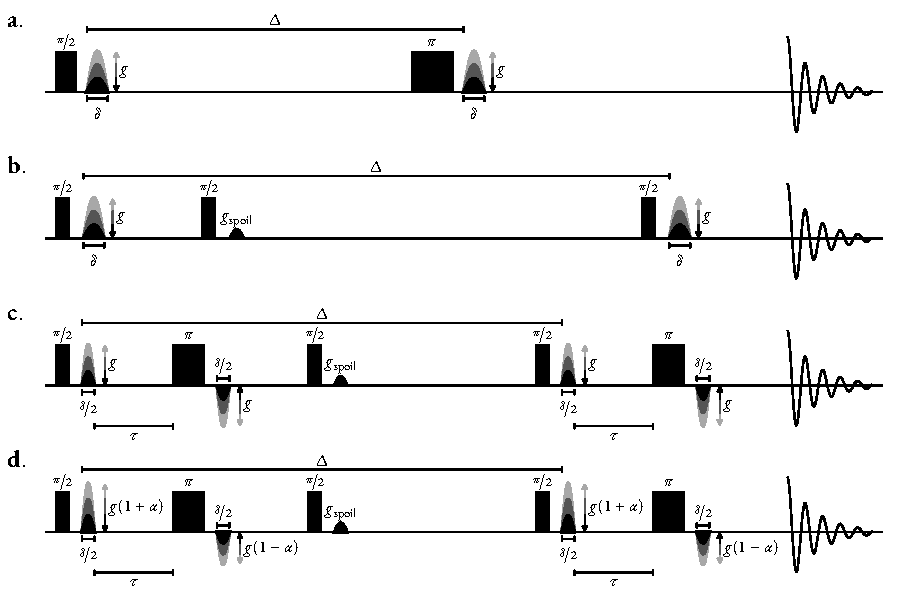
\includegraphics{diffusion_sequences/diffusion_sequences.pdf}
   \caption[
       Pulse sequences used for the determination of translational diffusion constants.
   ]{
       Pulse sequences used for the determination of translational diffusion constants.
       \textbf{a.} \acs{PGSE},
       \textbf{b.} \acs{PGSTE},
       \textbf{c.} \acs{PGSTEBP},
       \textbf{d.} One-shot DOSY.
       \ac{RF} pulses are denoted by solid rectangles. Diffusion-encoding
       gradients are denoted by sine-bell shapes with varying shades,
       indicating that the intensity ($g$) is incremented to create a \ac{2D}
       dataset. Spoiler gradients are denoted by solid black sine-bell shapes.
   }
   \label{fig:diffusion_sequences}
\end{figure}

Through consideration of the Bloch-Torrey equations, which
extend the classic Bloch equations to account for the effects of diffusion on
magnetisation~\cite{Torrey1956}, the following equation, known as the
\emph{Stejskal-Tanner equation}, may be derived:
\begin{equation}
    a(g) = a_0 \exp \left(- \gamma^2 \delta^2 g^2 D \left(\Updelta -
    \frac{\delta}{3}\right)\right),
    \label{eq:stejskal_tanner}
\end{equation}
where
$a_0$ is the amplitude of a given signal without the application of \acp{PFG},
$\delta$ is the duration of each \ac{PFG} (\unit{\second}), and
\correction{
    $\Updelta$ is the time from the start of the first \ac{PFG} to the start
    of the next,
}\label{corr:diffusion-time} often known as the \emph{diffusion time}
(\unit{\second}).
While \cref{eq:stejskal_tanner} is widely stated in the diffusion \ac{NMR}
literature, it is only strictly applicable when the \ac{PGSE} sequence is used,
and \acp{PFG} with rectangular amplitude profiles are applied\footnote{
    Rectangular \acp{PFG} (i.e. those in which there is an infinitesimal time
    to rise to full strength, and to fall back to zero) are technically
    impossible to achieve as they would require gradient coils with zero
    inductance, though in practice it is possible to generate gradients with
    behaviour close to this.
}. As will be discussed soon, the exact form of the pulse sequence impacts the
functional form by which $a(g)$ varies.

Tanner introduced a variant of the original \ac{PGSE} experiment called
\ac{PGSTE}~\cite{Tanner1970} (\cref{fig:diffusion_sequences}.b). Instead
of the diffusion period being bisected by a
\ang{180} pulse, \ac{PGSTE} features two \ang{90} pulses at the beginning and
end of the diffusion period.
Hence, the extent of signal loss due to relaxation is affected by $T_1$ in
\ac{PGSTE}, as opposed to $T_2$ in \ac{PGSE}. \ac{PGSTE} is therefore favoured
in scenarios where $T_1 \correction{\gg} T_2$\label{corr:t1-t2}, as improved data sensitivity is achievable.

Both \ac{PGSE} and \ac{PGSTE} employ \emph{monopolar} \acp{PFG} for diffusion
encoding.
Experiments also exist which employ
\emph{bipolar} gradient elements, which consist of a
\ac{PFG}, followed by a \ang{180} pulse, and then a second \ac{PFG} with the
opposite polarity to the first~\cite{Cotts1989,Wu1995}. The \ac{PGSTEBP} experiment
(\cref{fig:diffusion_sequences}.c) can be thought of as the bipolar analogue of
\ac{PGSTE}.
Bipolar gradients are useful in circumstances where it is important to purge
the effects of static gradients in the sample, caused by field inhomogeneities.
Morris and coworkers have developed the \emph{one-shot}
experiment~\cite{Pelta2002} (\cref{fig:diffusion_sequences}.d), which requires a
single transient per gradient strength (i.e. there is no requirement for a
phase-cycling scheme).  This is achieved through the use of bipolar gradients
which comprise asymmetrical \acp{PFG} with relative powers $1 + \alpha : 1 -
\alpha$ for some $\alpha \in (0, 1)$; commonly, $\alpha=0.2$.

The most common means of conducting a diffusion experiment is to run one of the
pulse sequences mentioned above (or variants thereof) with $g$ varied across
increments.
\correction{
    The \ac{FID}'s signal amplitudes always abide by the following general form
    of the Stejskal-Tanner equation, regardless of the exact pulse sequence
    used:
}\label{corr:stej-tann}
\begin{equation}
    a(g) = a_0 \exp\left(- c g^2 D\right),
\end{equation}
for some constant $c$ \correction{(\unit{\second\per\tesla\squared})}\label{corr:c-unit}.
The functional form of $c$ depends on the type of experiment used, as well as
the amplitude profile (\emph{shape}) of the \acp{PFG}.
A consideration of the Bloch-Torrey equations for a given experiment is
necessary, with an extensive overview provided by Sinnaeve for most diffusion
NMR experiments~\cite{Sinnaeve2012}. In general, $c$ is as follows:
\begin{equation}
    c = \gamma^2 \delta^2 \sigma^2 \Updelta^{\prime}.
    \label{eq:stejskal_tanner_generic}
\end{equation}
$\sigma$ is the \emph{shape factor} of the \acp{PFG} (\textit{vide infra}),
and $\Updelta^{\prime}$ is the effective time that diffusion is allowed
to occur. Examples of the form that $\Updelta^{\prime}$ takes include:
\begin{equation}
    \Updelta^{\prime} =
    \begin{cases}
        \Updelta + 2 \left(\kappa - \lambda\right) \delta &
        \text{\ac{PGSE}, \ac{PGSTE}}\\
        \Updelta + \frac{\left(2 \kappa - 2 \lambda - 1\right)\delta}{4} - \frac{\tau}{2} &
        \text{\ac{PGSTEBP}} \\
        \Updelta + \frac{\left(\kappa - \lambda\right)
            \left(\alpha^2 + 1\right) \delta}{2} +
        \frac{\left(\delta + 2 \tau\right)\left(\alpha^2 - 1\right)}{4} &
        \text{One-shot}
    \end{cases}.
    \label{eq:Delta-prime}
\end{equation}
$\tau$ is the delay between the initial \ac{PFG} and the \ang{180} pulse in
experiments with bipolar gradients.
The factors $\sigma$,  $\lambda$, and $\kappa$ are related to the shape
function $s(\epsilon) : \epsilon \in [0, 1]$ of the \ac{PFG}, which describes
the variation of the gradient amplitude as a function of its progression.
For a rectangular gradient, $s(\epsilon) = 1 \forall \epsilon$, whereas for a
sine-bell gradient, $s(\epsilon) = \sin(\pi \epsilon)$. The cumulative
distribution of the shape function is given by:
\begin{equation}
    S(\epsilon) = \int_0^{\epsilon} s\left(\epsilon^{\prime}\right)
            \mathrm{d} \epsilon^{\prime} \quad \forall \epsilon \in [0, 1].
\end{equation}
The corresponding definition of $S$ for a discrete gradient made of $N$
steps, $\symbf{s} \in \mathbb{R}^{N}$, is
\begin{equation}
    S_n =
        \frac{1}{n} \sum_{i = 1}^{n} s_i \quad
        \forall n \in \left\lbrace 1, \cdots, N\right\rbrace,
\end{equation}
$\sigma$, $\lambda$, and $\kappa$ are related to the shape function's
cumulative distribution as follows:
\begin{subequations}
    \begin{gather}
        \sigma = S(1),\\
        \lambda = \frac{1}{\sigma} \int_0^1 S(\epsilon) \mathrm{d} \epsilon,\\
        \kappa = \frac{1}{\sigma^2} \int_0^1 S^2(\epsilon) \mathrm{d} \epsilon,
    \end{gather}
\end{subequations}
with their discrete counterparts being:
\begin{subequations}
    \begin{gather}
        \sigma = S_{N} \\
        \lambda = \frac{1}{\sigma N} \sum_{n = 1}^{N} S_n
            = \frac{1}{\sigma N} \sum_{n=1}^{N}
            \left(\frac{1}{n} \sum_{i=1}^{n} s_i\right) \\
        \kappa = \frac{1}{\sigma^2 N} \sum_{n = 1}^{N} S^2_n
            = \frac{1}{\sigma^2 N} \sum_{n = 1}^{N}
            \left(\frac{1}{n} \sum_{i=1}^{n} s_i\right)^2.
    \end{gather}
\end{subequations}
For \acp{PFG} with a symmetrical shape, $\lambda = \nicefrac{1}{2}$. $\kappa$
is typically equal to or close to $\nicefrac{1}{3}$. It can now be seen that
the original Stejskal-Tanner equation for the
\ac{PGSE} experiment (\cref{eq:stejskal_tanner}) comes from
inserting \cref{eq:Delta-prime} into \cref{eq:stejskal_tanner_generic},
assuming a rectangular shape factor for the \acs{PFG}:
$\sigma = 1$,  $\lambda = \nicefrac{1}{2}$, and  $\kappa = \frac{1}{3}$.
In many situations,  $\Updelta$
dominates in the expression of $\Updelta^{\prime}$, and so ensuring the correct
form of $c$ could be seen as excessive. However, especially when  $\Updelta$ is
not orders of magnitude greater than $\delta$, the exact form of
$\Updelta^{\prime}$ used in \cref{eq:stejskal_tanner_generic} will be
important for accurate measurements of the diffusion coefficient.

\subsection{Analysing the Datasets}
Determining the quantity of interest from the above experiments is most
typically done using the following procedure:
\begin{enumerate}
    \item Each of the \acp{FID} in the series is processed using the same protocol,
        leading to a set of \ac{1D} spectra.
    \item Peak-picking is performed to locate the chemical shift values which
        correspond to signals of interest within the spectra.
    \item For each chemical shift corresponding to a peak location, the values
        of the spectra are extracted across increments. The relevant
        function describing how the amplitude is expected to decay across
        increments is then fit to these values, to extract the quantity of
        interest.
\end{enumerate}
This method is \emph{univariate} in the sense that it considers a single sample
(chemical shift) in isolation from the rest of the data.
It is popular to visualise the result of univariate fitting by plotting \ac{2D}
pseudo-spectra, featuring axes denoting (a) chemical shift, and (b)
the parameter of interest. Distributions taking
into account the predicted value of interest and the associated uncertainty
are plotted at each chemical shift.
In the context of diffusion \ac{NMR}, this form of data analysis is
referred to as \ac{DOSY}~\cite{Morris2009b}.
The \ac{DOSY} approach works well in cases where peaks of interest are intense
and well-resolved. However, when there is considerable peak overlap, accurately
determining the parameter of interest associated with a given signal becomes
more challenging, since nearby signals will influence the rate of amplitude
decay. An aggregated value of the decay rates of the contributing signals
will be predicted using the above approach.
In such cases, it is possible to instead fit
a superposition of functions to the spectral amplitudes, as a means of
separating out contributions from the overlapping signals~\cite{Nilsson2006}.
However, this process is usually only effective when the data has very high
\ac{SNR}, and the quantities of interest associated with the overlapping
signals differ considerably.

An alternative approach
is to use a \emph{multivariate} analysis, in which entire spectrum is
considered holistically, and an attempt is made to decompose the spectrum into
components with different decay rates. Prominent examples of multivariate methods
developed for diffusion data analysis are \ac{DECRA}~\cite{Windig1998} and
\emph{speedy} component resolution (\acs{SCORE})~\cite{Nilsson2008}, an
improvement of the original \acs{CORE}~\cite{Stilbs1996,Stilbs1996b}.
\acused{SCORE}\acused{CORE}
Multivariate techniques tend to only be effective in situations where a
few (2 or 3) different signal decay rates are present. In diffusion
\ac{NMR}, each molecule in the sample will give rise to the same decay rate
across its signals (effects such as chemical exchange can lead to exceptions to
this: \cref{fig:andrographolide-dosy} provides an example of this). As such,
only a few decay rates typically govern the form of diffusion data, making
multivariate approaches feasible.
Conversely, multivariate methods are generally unsuitable for inversion
recovery and \ac{CPMG} datasets: each spin in a sample will possess different
$T_1$ and $T_2$ values, such that a far greater number of decay rates will be
present.

\subsection{Methodology}
\label{subsec:seq-method}
A straightforward extension of \ac{1D} parametric estimation
provides a route to estimating amplitude-attenuated datasets in a
fashion with similarities to the traditional univariate (\ac{DOSY}) approach.
The theory of this method will now be discussed.

Suppose one of the experiments mentioned above is run with $K \in \mathbb{N}$
increments,
such that there is a vector  $\symbf{p} \in \mathbb{R}^K$ comprising the
values of the pulse sequence variable used to acquire each \ac{1D} \ac{FID} in
the data.  The complete dataset is expected to take the form $\symbf{Y} \in
\mathbb{C}^{K \times N}$ in which the value of the pulse sequence variable
affects the amplitudes of the contributing signals:
\begin{equation}
    \begin{gathered}
        y_{k,n} = \sum_{m=1}^{M} a_{k,m} \exp(\iu \phi_m)
        \exp((2 \pi \iu (f_m - \foff) - \eta_m) n \Dt),\\
        \forall k \in \lbrace 1, \cdots, K \rbrace,\ \forall n \in \lbrace 0,
        \cdots, N-1 \rbrace.
    \end{gathered}
\end{equation}
$\symbf{A} \in \mathbb{R}^{K \times M}$ is a matrix of the signal amplitudes
across the \acp{FID}:
\begin{equation}
    \symbf{A} =
    \begin{bmatrix}
        a_{1,1} & a_{1,2} & \cdots & a_{1,M}\\
        a_{2,1} & a_{2,2} & \cdots & a_{2,M}\\
        \vdots & \vdots & \ddots & \vdots\\
        a_{K,1} & a_{K,2} & \cdots & a_{K,M}
    \end{bmatrix}
\end{equation}
A complete parameter vector for the dataset is given by $\bth \in
\mathbb{R}^{(K + 3)M}$:
\begin{equation}
    \bth =
    \begin{bmatrix}
        \symbf{a}_1 & \cdots & \symbf{a}_K & \bdphi\T & \bdf\T & \bdeta\T
    \end{bmatrix}\T,
\end{equation}
where $\symbf{a}_k \in \mathbb{R}^M$ denotes the relevant row in $\symbf{A}$.
The amplitudes are a function of the pulse sequence variable with the following
form:
\begin{equation}
    a_{k,m} = a_{0,m} \mathcal{A} (\psi_m \hspace*{2pt} | \hspace*{2pt} p_k).
\end{equation}
$\symbf{a}_0 \in \mathbb{R}^{M}$ is a vector of the ``maximal
amplitudes'' of the signals, and $\symbf{\psi} \in \mathbb{R}^M$ is a vector
of the parameter of interest ($T_1$,  $T_2$, $D$) associated with
each signal. $a_{0,m}$ can be thought of as the largest
possible amplitude that could be obtained for signal $m$ with the given
pulse sequence:
\begin{itemize}
    \item In an inversion recovery experiment, the largest amplitude is
        achieved as $\tau \rightarrow \infty$, as the spin system will have
        returned back to equilibrium prior to the \ang{90} pulse.
    \item With \ac{CPMG} experiments, the largest amplitude will occur when
        $n = 0$, as no time is designated for transverse
        relaxation to take place.
    \item For diffusion experiments, the largest amplitude is achieved when
        $g=0$, since no diffusion-induced dephasing of spins will have
        occurred.
\end{itemize}
The function $\mathcal{A}$ describes how the amplitudes of signals are
attenuated by the experimental variable, and has a form which is intimately
linked to the type of experiment. For the experiments described in
\cref{subsec:relaxation_experiments,subsec:diffusion_experiments},
the forms of $\mathcal{A}$ are listed in \cref{tab:seq-equations}.
\begin{table}
    \begin{center}
        \begin{tabular}{ccccccc}
            \hline
            Experiment &
            $p$ &
            $\psi$ &
            $\mathcal{A}(\psi | p)$ &
            $\frac{\partial \mathcal{A}(\psi | p)}{\partial \psi}$ &
            $\frac{\partial^2 \mathcal{A}(\psi | p)}{\partial \psi^2}$ \\ \hline
            Inv. Recov.&
            $\tau$ &
            $T_1$ &
            $\left(1 - 2 \exp \left(-\frac{\tau}{T_{1}}\right)\right)$ &
            $-\frac{2 \tau}{T_1^2} \exp\left(-\frac{\tau}{T_1}\right)$ &
            $\frac{2 \tau}{T_1^3} \exp\left(-\frac{\tau}{T_1}\right)\left(2 - \frac{\tau}{T_1}\right)$\\
            \acs{CPMG} &
            $n$ &
            $T_2$ &
            $\exp\left(-\frac{2 \tau n}{T_2}\right)$ &
            $\frac{2 \tau n}{T_2^2}\exp\left(-\frac{2 \tau n}{T_2}\right)$ &
            $\frac{2 \tau n}{T_2^3}\exp\left(-\frac{2 \tau n}{T_2}\right)
            \left( \frac{2 \tau n}{T_2} - 2 \right)$ \\
            Diffusion &
            $g$ &
            $D$ &
            $\exp\left(-c g^2 D\right)$ &
            $-c g^2 \exp\left(-c g^2 D\right)$ &
            $c^2 g^4 \exp\left(-c g^2 D\right)$ \\
            \hline
       \end{tabular}
       \caption[
           The various functional forms of $\mathcal{A}$ according to the
           different amplitude-attenuating NMR experiments considered.
       ]
       {
           The various functional forms of $\mathcal{A}$ according to the
           different amplitude-attenuating NMR experiments considered, along
           with the first and second derivatives, which are required to extract
           estimates of $\psi$ using \ac{NLP}.
       }
       \label{tab:seq-equations}
    \end{center}
\end{table}

\subsubsection{Estimating the Datasets}
The close relationship between the \acp{FID} within the dataset means that
completely estimating all of them separately, without exploiting information
from previously estimated \acp{FID}, is unnecessary.
Instead, after the first increment is estimated without prior knowledge,
yielding $\bth_{1} \in \mathbb{R}^{4M}$, the phases, frequencies and damping
factors, all of which are anticipated to remain the same across the
\acp{FID}, are fixed.
Subsequent parameter estimates are determined by taking the result from
the previous \ac{FID}, and subjecting it to \iac{NLP} routine in which only
the amplitudes are optimised. Thus, estimating each subsequent iteration
is reduced to the problem\footnote{
    $\mathcal{F}$ in \cref{eq:fidelity-amp} reads as ``the fidelity
    with respect to the amplitudes $\bda$, given phases $\bdphi_{1}$,
    frequencies $\bdf_{1}$, damping factors  $\bdeta_{1}$, and \ac{FID}
    $\by_k$''. The fidelity has exactly the same mathematical form as
    \cref{eq:fidelity}, though it has been emphasised that the phases,
    frequencies and damping factors are no longer variables to be optimised,
    but fixed parameters.
}
\begin{equation}
    \symbf{a}_k = \argmin_{\bda \in \mathbb{R}^M}
        \mathcal{F}(\bda \hspace*{2pt} | \hspace*{2pt}
        \bdphi_{1}, \bdf_{1}, \bdeta_{1}, \by_k)\quad\forall k \in \lbrace2, \cdots, K\rbrace.
        \label{eq:fidelity-amp}
\end{equation}
\Iac{NLP} routine can solve this very efficiently, typically in a few
iterations, on account of the linear dependence of the model with respect to
the oscillator amplitudes. The linear dependence means that second
derivatives of the model are all zero (see \cref{eq:amp-second-deriv}),
such that only first derivatives need to be computed to derive an exact Hessian
matrix of the fidelity.
Due to the linear dependence on amplitudes, an alternative means of
deriving amplitudes for each increment is to compute the following:
\begin{subequations}
    \begin{gather}
        \symbf{a}_k = \symbf{Z}^+ \symbf{y}_k, \\
        \symbf{Z} =
        \begin{bmatrix}
            1 & \cdots & 1 \\
            z_1 & \cdots & z_M\\
            \vdots & \ddots & \vdots \\
            z_1^{N-1} & \cdots & z_M^{N-1}
        \end{bmatrix}
        \begin{bmatrix}
            \exp(\iu \phi_1) \\ \vdots \\ \exp(\iu \phi_M)
        \end{bmatrix},\\
        z_m = \exp((2\pi \iu (f_m - \foff) - \eta_m)\Dt).
    \end{gather}
\end{subequations}
An outline of the estimation procedure is provided by \cref{alg:estimate-seq}.

\begin{algorithm}
    \caption[
        The proposed routine for estimating a sequence of amplitude-attenuated
        \acsp{FID}.
    ]
    {
        The proposed routine for estimating a sequence of amplitude-attenuated
        \acsp{FID}.
        \textsc{NLPAmp} denotes a
        routine which is akin to \textsc{NLP} (\cref{alg:nlp}), except
        only amplitudes are optimised; phases, frequencies and damping factors
        are fixed.
    }
    \label{alg:estimate-seq}
    \begin{algorithmic}[1]
        \Procedure{EstimateAmpAttenuated}{
            $\bY \in \mathbb{C}^{K \times N},
            l_{\text{I}},
            r_{\text{I}},
            l_{\text{N}},
            r_{\text{N}},
            \chi \in \mathbb{R}_{>1},
            M \in \mathbb{N}_0$
        }
        \State $\bth_{1}, \symbf{\epsilon}_{1} \gets \textsc{Estimate$1$D}\left(
            \by_1,
            l_{\text{I}},
            r_{\text{I}},
            l_{\text{N}},
            r_{\text{N}},
            \chi,
            M
            \right)
        $;
        \Comment{Estimate first increment, see \cref{alg:1d-2d-summary}.}
        \State $M \gets \nicefrac{\text{len}(\bth_{1})}{4}$;
        \State $\bth, \symbf{\epsilon} \gets  \symbf{0} \in \mathbb{R}^{(K + 3)M}, \symbf{0} \in \mathbb{R}^{(K + 3)M}$;
        \Comment{Initialise complete parameter vector.}
        \State $\bth[:M], \symbf{\epsilon}[:M] \gets \bth_{1}[:M], \symbf{\epsilon}_{1}[:M]$;
        \Comment{Amplitudes for first increment.}
        \State $\bth[KM:], \symbf{\epsilon}[KM:] \gets \bth_{1}[M:], \symbf{\epsilon}_{1}[M:]$;
        \Comment{Phases, frequencies and damping factors, which are fixed.}
        \For{$k=2, \cdots, K$}
            \State $\widetilde{\by} \gets \textsc{Filter$1$D}\left(
                \by_k,
                l_{\text{I}},
                r_{\text{I}},
                l_{\text{N}},
                r_{\text{N}},
                \chi,
                \right);
                $
            \Comment{\cref{alg:filter-1d}.}
            \State $\bth_{k}, \symbf{\epsilon}_{k} \gets
            \textsc{NLPAmp}\left(\widetilde{\by}, \bth_{k-1}\right)$;
            \Comment{Similar to \cref{alg:nlp}, though see the caption.}
            \State $\bth[kM : (k+1)M], \symbf{\epsilon}[kM : (k+1)M] \gets \bth_k[:M], \symbf{\epsilon}_k[:M]$;
            \Comment{Extract amplitudes.}
        \EndFor
        \State \textbf{return} $\bth, \symbf{\epsilon}$;
        \EndProcedure
    \end{algorithmic}
\end{algorithm}



\subsubsection{Determining the Parameter of Interest}
Having generated a parameter estimate for each \ac{FID} in the dataset, focus
now moves to determining the parameter of interest for each signal.
For each oscillator $m \in \lbrace 1, \cdots, M \rbrace$, the maximal amplitude
and parameter of interest are determined by solving the following problem:
\begin{subequations}
    \begin{gather}
        \symbf{\vartheta}_m^{(*)} = \argmin_{\symbf{\vartheta} \in \mathbb{R}^2}
        \left\lVert
            \symbf{a}_m - a_0 \mathcal{A} \left(\psi \hspace*{2pt} | \hspace*{2pt} \symbf{p}\right)
        \right\rVert^2,\\
        \symbf{\vartheta} = \left[ a_0 \hspace{10pt} \psi \right]\T \implies
        \symbf{\vartheta}_{m}^{(*)} = \left[ a_{0,m}^{(*)}  \hspace{10pt} \psi_{m}^{(*)} \right]\T,
    \end{gather}
\end{subequations}
where $\symbf{a}_m$ corresponds to the $m$\textsuperscript{th} column of
$\symbf{A}$.  This is another example of \iac{RSS} problem, which can be solved using
\iac{NLP} routine as already described. The gradient vector and Hessian matrix
of the fidelity take very similar functional forms to those for \ac{FID}
estimation for this reason (see \cref{eq:grad,eq:hess}), and are as
follows $\forall
i, j \in \lbrace 1, 2 \rbrace$:
\begin{subequations}
    \begin{gather}
        g(\symbf{\vartheta})_i =
            -2 \left \langle
                \symbf{a}_m - a_0 \mathcal{A}(\psi | \symbf{p}),
                \frac{\partial a_0 \mathcal{A} (\psi | \symbf{p})}
                {\partial \vartheta_i}
            \right \rangle,\\
        h(\symbf{\vartheta})_{i,j} =
            2 \left( \left \langle
                \frac{\partial a_0 \mathcal{A} (\psi | \symbf{p})}{\partial \vartheta_i},
                \frac{\partial a_0 \mathcal{A} (\psi | \symbf{p})}{\partial \vartheta_j}
            \right \rangle -
            \left \langle
                \symbf{a}_m - a_0 \mathcal{A}(\psi | \symbf{p}),
                \frac{\partial^2 a_0 \mathcal{A} (\psi | \symbf{p})}{\partial
                \vartheta_i\partial \vartheta_j}
            \right \rangle \right),
            \label{eq:seq-hessian}\\
    \end{gather}
\end{subequations}
with explicit expressions for the requisite first and second derivatives being
\begin{subequations}
    \begin{gather}
        \frac{\partial a_0 \mathcal{A} (\psi | \symbf{p})}{\partial a_0} =
            \mathcal{A} (\psi | \symbf{p}),\\
        \frac{\partial a_0 \mathcal{A} (\psi | \symbf{p})}{\partial \psi} =
            a_0 \frac{\partial \mathcal{A} (\psi | \symbf{p})}{\partial \psi},\\
        \frac{\partial^2 a_0 \mathcal{A} (\psi | \symbf{p})}{\partial a_0^2} = 0,\\
        \frac{\partial^2 a_0 \mathcal{A} (\psi | \symbf{p})}{\partial \psi^2} =
            a_0 \frac{\partial^2 \mathcal{A} (\psi | \symbf{p})}{\partial \psi^2},\\
        \frac{\partial^2 a_0 \mathcal{A} (\psi | \symbf{p})}{\partial a_0 \partial \psi} =
            \frac{\partial^2 a_0 \mathcal{A} (\psi | \symbf{p})}{\partial \psi \partial a_0} =
            \frac{\partial \mathcal{A} (\psi | \symbf{p})}{\partial \psi}.
    \end{gather}
\end{subequations}
The functional forms of the first and second derivatives of $\mathcal{A}$ for
the different experiments of interest are given in \cref{tab:seq-equations}.

\subsubsection{Displaying Results}
It is possible to visualise the estimation results acquired by this method in a
similar fashion to \ac{DOSY} analysis. For each oscillator in the estimated
model, a \ac{2D} array is generated, corresponding to the outer product of the
\ac{FT} of the model oscillator ($\symbf{s}_m$) and a distribution describing
the predicted value of $\psi$ ($\symbf{d}_m$).
\begin{subequations}
    \begin{gather}
        \mathbb{R}^{R \times N} \ni \symbf{S} = \sum_{m=1}^{M}
        \symbf{d}_m \otimes
        \symbf{s}_m ,\label{eq:dosy-spectrum}\\
        \symbf{s}_m = \Re\left(\FT\left(\bx_m\right)\right),\\
        x_{m,n} = a_{0,m} \exp(\iu \phi_m)
        \exp((2 \pi \iu (f_m - \foff) - \eta_m ) n \Dt),
    \end{gather}%
    \label{eq:dosy-cross-product}%
\end{subequations}
where $R \in \mathbb{N}$ is the number of samples to generate the distribution from.
The exact form that the distribution $\symbf{d}_m$ should take is arbitrary,
though it should indicate two key pieces of information:
\begin{itemize}
    \item Its maximum should coincide with the predicted value of $\psi_m$.
    \item Its broadness should indicate the level of uncertainty associated
        with the prediction.
\end{itemize}
In this work, the distribution used is a Gaussian distribution with mean
$\psi_m$ and standard deviation $c \epsilon_m$, where $\epsilon_m$ is the
estimation error associated with oscillator $m$'s parameter of interest, and $c
\in \mathbb{R}_{>0}$ is an arbitrary broadening factor which can be chosen to
ensure clear visibility of
the peaks\footnote{
    In cases where the error in estimating $\psi_m$ is very small, it may be
    that the distribution derived from \cref{eq:distribution} satisfies
    $\text{max}(\symbf{d}_m)=0$ if the peak of the distribution does
    not closely coincide with any of the sampled values. The affected
    oscillator will not appear in the \ac{DOSY}-like spectrum under these
    circumstances.
    Broadening the distribution (i.e. setting $c > 1$) resolves this.
}:
\begin{subequations}
    \begin{gather}
        d_{m,r} = \frac{1}{\sqrt{2 \pi (c \epsilon_m)^2}}
        \exp\left(
            - \frac{(p_r - \psi_m)^2}{2 (c \epsilon_m)^2}
        \right)\quad \forall r \in \lbrace 1, \cdots, R \rbrace,\\
        p_r = p_{\text{min}} + \frac{(r-1) (p_{\text{max}} - p_{\text{min}})}{R-1}.
    \end{gather}
    \label{eq:distribution}%
\end{subequations}
$p_{\text{min}}$ and $p_{\text{max}}$ specify the range of values over which to
generate the distribution.
\correction{
    The errors associated with the parameter of interest can be determined as
    follows:
    \begin{equation}
        \epsilon_m = \sqrt{
            \frac{
                \left\lVert \symbf{a}_{m} - a_{0,m}^{(*)} \mathcal{A}\left(\psi_{m}^{(*)} \big\vert \hspace*{1pt}\symbf{p}\right) \right\rVert^2
                \left[\symbf{H}\left(\symbf{\vartheta}_{m}^{(*)}\right)^{-1}\right]_{2,2}
            }
            {K-1}
        },
        \label{eq:seq-errors}
    \end{equation}
    where $\symbf{H}\left(\symbf{\vartheta}_m^{(*)}\right) \in \mathbb{C}^{2 \times
    2}$ is the Hessian at convergence, comprising elements of the form
    $h\left(\symbf{\vartheta}_m^{(*)}\right)_{i,j}$ (see \cref{eq:seq-hessian}).
    The derivation of \cref{eq:seq-errors} is akin to that for the errors associated
    with \ac{FID} estimation; more detail on \ac{FID} estimation errors is
    provided in \cref{subsec:errors}.
}\label{corr:seq-errors}

\subsection{Results}
\label{subsec:seq-results}
\subsubsection{``Five Multiplets''}
\begin{figure}
    \vspace{-10pt}
    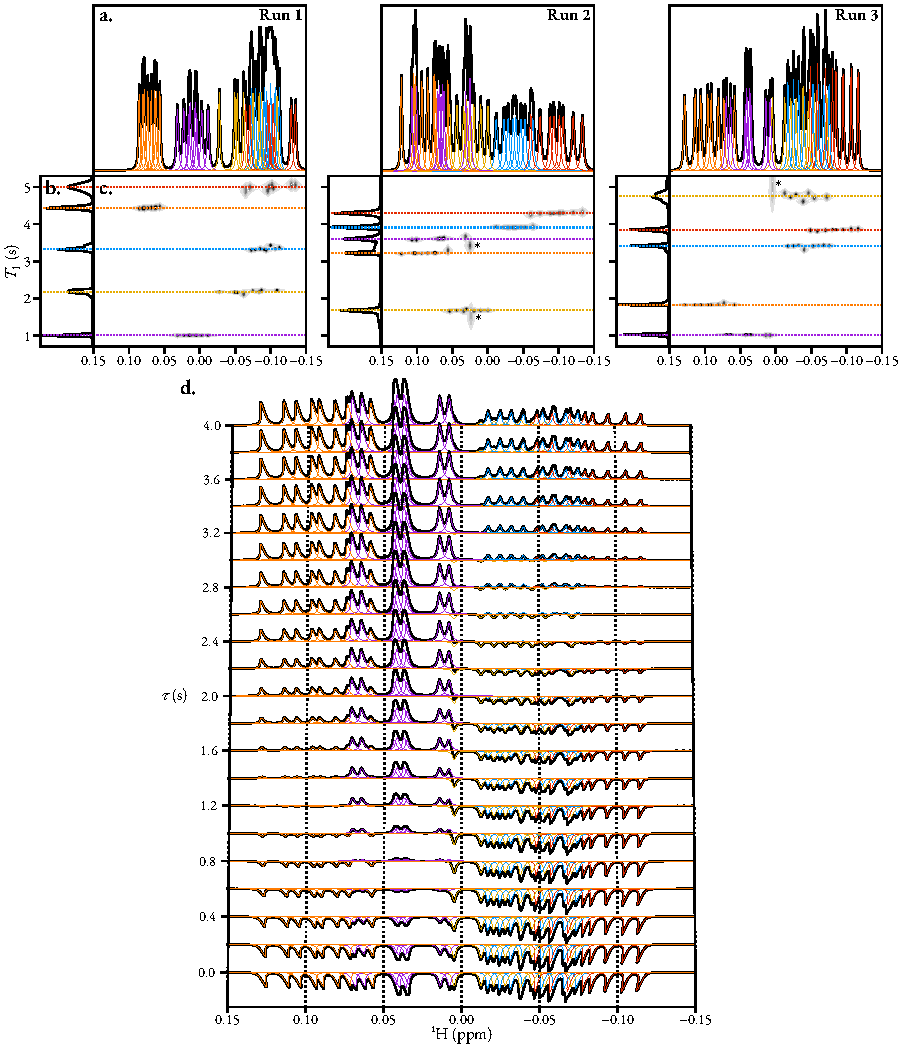
\includegraphics{five_multiplets_invrec/five_multiplets_invrec.pdf}
    \caption[
        Three examples of results generated when considering simulated
        inversion recovery datasets comprising five ddd multiplet structures.
    ]
    {
        Three examples of results generated when considering
        simulated inversion recovery datasets comprising five ddd multiplet
        structures.
        \textbf{a.} Plot of the result generated for the first increment ($\tau
        = \qty{0}{\second}$), with all the plots multiplied by $-1$. Black:
        spectrum of the data. Coloured lines: peaks corresponding to
        oscillators in the estimated model. Oscillators with the same colour
        are components of the same multiplet.
        \textbf{b.} Distribution of $T_1$ values, generated
        by projecting the array in panel c onto the $y$-axis.
        \textbf{c.} \ac{DOSY}-style representation of the result, generated using
        \cref{eq:dosy-cross-product},
        with
        $p_{\text{min}} = \qty{0.7}{\second}$,
        $p_{\text{max}} = \qty{5.3}{\second}$,
        $c = 40$,
        $R=128$.
        Dashed horizontal lines denote the true $T_1$ values for each spin.
        \textbf{d.} Estimation result of each increment for Run 3,
        illustrating the evolution of the amplitudes of each oscillator as a
        function of $\tau$.
    }
    \label{fig:five-multiplets-invrec}
\end{figure}
\Cref{fig:five-multiplets-invrec} shows the result achieved by applying the
method outlined in \cref{alg:estimate-seq}
to three simulated inversion recovery datasets featuring 5 overlapping ddd
multiplet structures.
Each dataset was simulated using \textsc{Spinach}, using spin systems which
were defined such that within a
known region of the generated spectrum
(\SIrange{0.15}{-0.15}{\partspermillion}) five ddd
multiplet structures with significant overlap, abiding by the weak coupling
approximation, were present.
Constraints were placed on the shifts and
couplings of the spin system to ensure that no two signals would have
frequencies with a difference less than $\nicefrac{\fswone}{\None}$.
For each spin, a $T_1$ value was sampled from $\mathcal{U}(\qty{1}{\second},
\qty{5}{\second})$, and a $T_2$ value was sampled from
$\mathcal{U}(\qty{0.2}{\second}, \qty{0.6}{\second})$.
Relaxation phenomena were modelled using the ``extended $T_1$/$T_2$
approximation''~\cite{SpinachRelax} (see \cref{subsec:invrec-datasets} for more
information).
Each \ac{FID} generated dataset was corrupted by noise with a target
\ac{SNR} of \qty{40}{\deci\bel}. The \ac{MDL} was used for model order
prediction; it successfully predicted that 40 signals were present on each
occasion.

Despite heavy overlap between peaks, the routine was successful at
assigning each signal in the dataset with a $T_1$ value that closely agreed
with the $T_1$ of the spin giving rise to it (see
\cref{fig:five-multiplets-invrec}.b). As is to be
expected, in scenarios where little overlap existed between signals with
different decay rates, $T_1$ predictions tended to be more accurate, with
smaller associated errors (see for example the purple and orange multiplets in Run 1.
Nevertheless, good estimates could still be obtained in cases of severe
overlap between signals from different spins (see the red, blue and yellow
multiplets in Run 1). Reassuringly, particular oscillators for which the
estimate of $T_1$ was notably far from the true value tended to be associated
with large errors, with examples denoted with an asterisk in
\cref{fig:five-multiplets-invrec}.c.

\subsubsection{Andrographolide Diffusion}
\begin{figure}
    \centering
    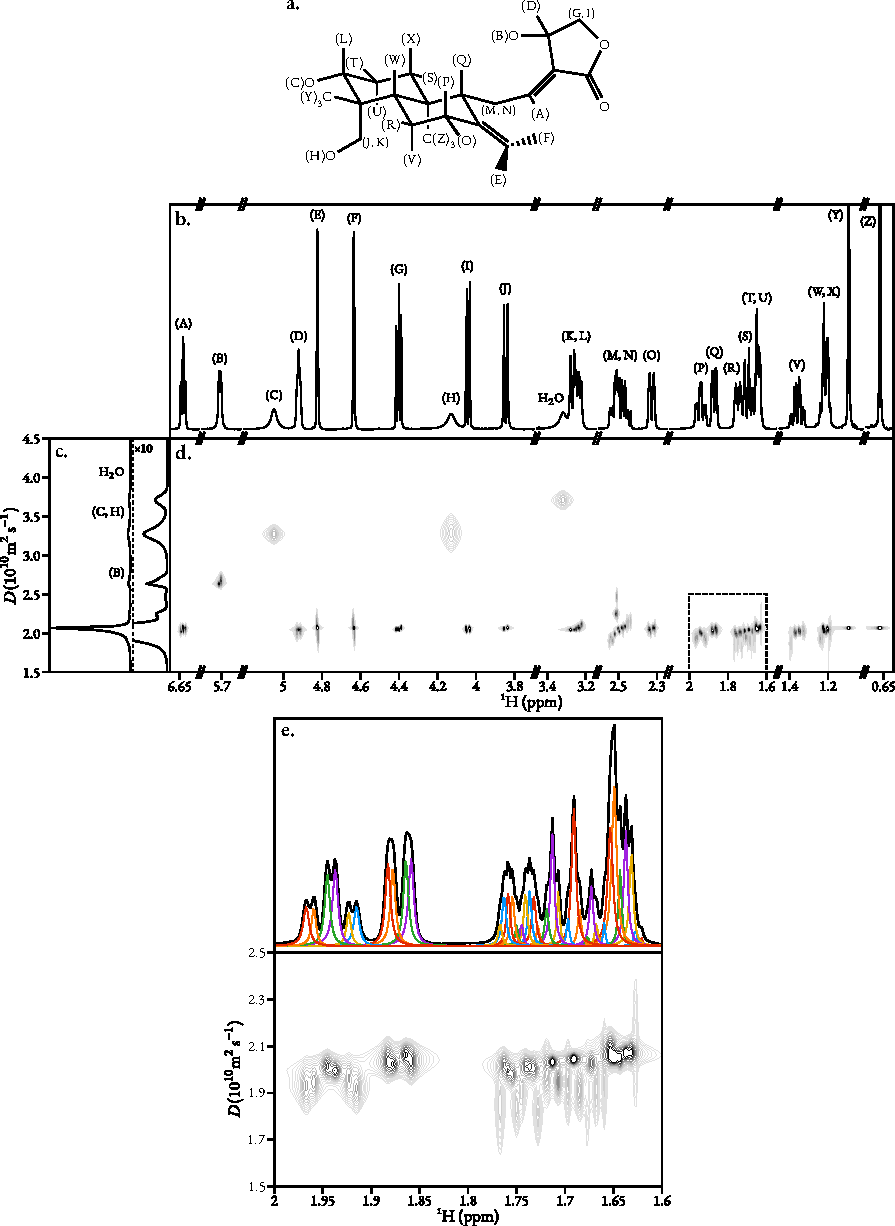
\includegraphics{andrographolide_dosy/andrographolide_dosy.pdf}
    \caption[
        The result of estimating a diffusion dataset of andrographolide.
    ]{
        The result of estimating a diffusion dataset of andrographolide in
        unfresh \acs{DMSOd6}.
        \textbf{a.} Structure of andrographolide.
        \textbf{b.} \ac{1D} spectrum.
        \textbf{c.} Diffusion profile obtained by projecting the contour plot in
        c onto the $y$-axis.
        \textbf{d.} Contour plot mapping estimated oscillators to diffusion constants, with
        $p_{\text{min}} = \qty{1.5e-10}{\meter\squared\per\second}$,
        $p_{\text{max}} = \qty{4.5e-10}{\meter\squared\per\second}$,
        $c = 2.5$,
        $R=128$.
        \textbf{e.} Magnified view of the \SIrange{2}{1.6}{\partspermillion}
        spectral range (see the dashed box in panel d) with estimated
        oscillator peaks plotted.
    }
    \label{fig:andrographolide-dosy}
\end{figure}
\Cref{fig:andrographolide-dosy} shows the result of applying the
estimation technique on a oneshot \ac{DOSY} dataset of andrographolide in
unfresh \acs{DMSOd6} at \qty{298}{\kelvin}. Exposure of the sample to water is
evidenced by the broad
peak around \qty{3.3}{\partspermillion}, estimated to have a diffusion constant
of \qty{3.7e-10}{\meter\squared\per\second}. On top of this, the acidic
hydroxyl protons (B, C, H) of andrographolide show significant line-broadening,
and their estimated diffusion coefficients are considerably different compared
with those of the non-hydroxyl protons, due chemical exchange with water in the
sample~\cite{Chen1998}.
The diffusion profile generated suggests a diffusion constant of andrographolide of
\qty{2.07e-10}{\meter\squared\per\second}. The predicted diffusion constants for
each estimated oscillator, especially those with greater intensity, show
good consistency.
Lower intensity oscillators, especially those which
significantly overlap with others, tended to be associated with
less consistent diffusion constants and larger errors with examples of this
phenomenon apparent in \cref{fig:andrographolide-dosy}.d. A few
oscillators also show a
significant deviation at around \qty{2.5}{\partspermillion}. This is due to the
presence of a 1:2:3:2:1 quintet from partially protonated \acs{DMSO}, due to
proton exchange with the residual water\footnote{
    This multiplet structure arises from the \ch{^1H} in \acs{DMSO} coupling to
    two
    equivalent spin-$1$ \ch{^2H} nuclei. The relative amplitudes of the signals
    can be deduced by considering the ``trinomial triangle'', an extension of
    the more familiar Pascal's triangle, the latter being applicable to
    couplings involving equivalent spin-$\nicefrac{1}{2}$ nuclei.
}. As the
data are insufficiently resolved to enable the separation of andrographoilde and
\acs{DMSO} signals, oscillators exist in the model which have amplitude profiles
influenced by both species, leading to an aggregated diffusion constant. As
$D_{\text{DMSO}} > D_{\text{andrographoilide}}$, the affected oscillators
possess larger predicted diffusion constants.

\subsubsection{Glucose/Valine/Threonine Diffusion}
\begin{figure}
    \centering
    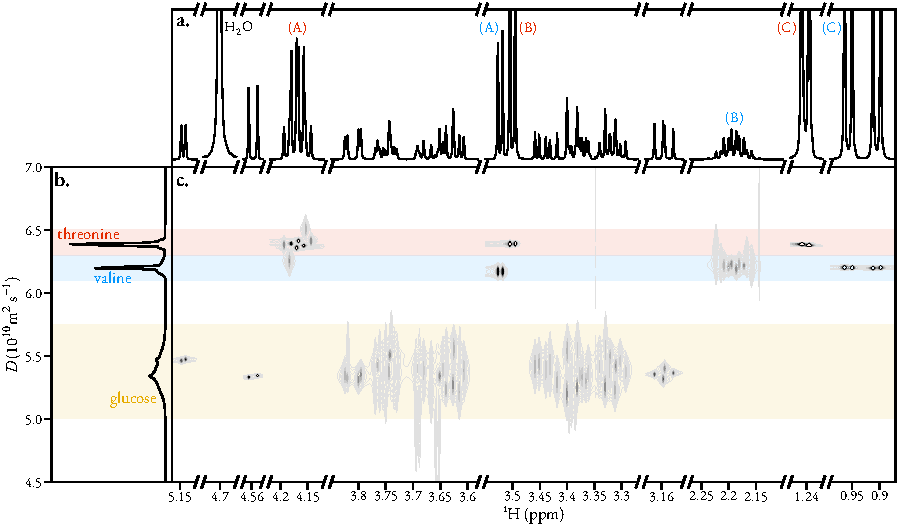
\includegraphics{glu_thre_val_diffusion/glu_thre_val_diffusion.pdf}
    \caption[
        The result of estimating a diffusion dataset for a mixture of L-threonine,
        L-valine and D-(+)-glucose.
    ]{
        The result of estimating a diffusion dataset for a mixture of L-threonine,
        L-valine and D-(+)-glucose in D\textsubscript{2}O.
        \textbf{a.} Structure of L-valine.
        \textbf{b.} Structure of L-threonine.
        \textbf{c1.} Structure of \textalpha-D-glucopyroanose.
        \textbf{c2.} Structure of \textbeta-D-glucopyroanose.
        \textbf{d.} \acs{1D} spectrum, taken from the first \acs{FID} of the
        diffusion dataset.
        \textbf{e.} Diffusion coefficient distribution.
        \textbf{f.} \acs{DOSY}-style plot of chemical shifts vs diffusion
        constant, generated using \cref{eq:distribution}, with
        $p_{\text{min}} = \qty{4.5e-10}{\meter\squared\per\second}$,
        $p_{\text{max}} = \qty{7e-10}{\meter\squared\per\second}$,
        $R=256$, and $c=1.5$.
    }
    \label{fig:gluc_val_thre}
\end{figure}
Another diffusion example is provided by \cref{fig:gluc_val_thre}, where the
estimation routine was applied to a dataset derived from a sample comprising
the molecules L-valine ($M_r = \qty{117.148}{\gram\per\mole}$),
L-threonine ($M_r = \qty{119.120}{\gram\per\mole}$), and D-(+)-glucose ($M_r =
\qty{180.156}{\gram\per\mole}$) dissolved in
D\textsubscript{2}O at \qty{298}{\kelvin}. Not included in the figure is the
result for the water signal, for which a diffusion constant of
\qty{1.88e-9}{\meter\squared\per\second} was determined. The routine
was able to separate of the three species in the sample along the diffusion
axis. Predicted diffusion coefficients for valine and threonine were
\qty{6.20e-10}{\meter\squared\per\second} and
\qty{6.39e-10}{\meter\squared\per\second}, respectively. For glucose, the situation is
complicated by the presence of two major anomeric forms:
\textalpha-D-glucopyroanose and
\textbeta-D-glucopyroanose\footnote{
    The equilibrium mixture in water comprises 38\% of the \textalpha\ isomer
    and 62\% of the \textbeta\ isomer.
    This is evidenced by the
    spectrum in \cref{fig:gluc_val_thre}.a, where the relative integrals of
    the doublets at \qty{5.15}{\partspermillion} and
    \qty{4.56}{\partspermillion} agree with this ratio.
    A tiny amount of the open-chain form will
    also be present, though in a negligible quantity.
}~\cite[Chapter 3]{Davis2002}.
There is some evidence of separation of these anomers, principally due
to the downfield doublets at \qty{5.15}{\partspermillion} (\textalpha-anomer) and
\qty{4.56}{\partspermillion} (\textbeta-anomer), which have estimated diffusion
coefficients of \qty{5.47e-10}{\meter\squared\per\second}
and \qty{5.34e-10}{\meter\squared\per\second}, respectively. Beyond these
however, the other estimated oscillators corresponding to glucose have
associated errors which are too large for clear resolution of the two species.
\correction{
    The small difference in diffusion constants associated with the anomers is
    likely related to how effectively they are able to hydrogen-bond to the
    solvent.
}\label{corr:gluc-D}

As is to be expected, signals which are of greater intensity, and which are
more clearly resolved, enable the determination of diffusion coefficients with
smaller associated errors. A clear example of this behaviour can be recognised when
considering the valine result (see the area shaded blue in
\cref{fig:gluc_val_thre}.c). The
oscillators which lead to diffusion constants with the lowest errors correspond to
the high intensity doublet of doublets around \qty{0.95}{\partspermillion},
resulting from six equivalent protons from two methyl groups. Far
greater uncertainty is observed for the predictions associated with proton (B),
which has a doublet of septets structure, featuring many low-intensity signals.
Similar arguments can be made for the signals which correspond to the other
species in the mixture.
Application of multivariate methods on the dataset was unsuccessful at
extracting diffusion information for the separate components; both
\ac{DECRA} and \ac{SCORE} could extract the water
signal from the rest of the dataset, with the two components having associated
diffusion coefficients of \qty{6.31e-10}{\meter\squared\per\second} (an
aggregate of the valine, threonine, and glucose signals) and
\qty{1.88e-9}{\meter\squared\per\second}, respectively.

\section{Ideal Spectra from Single-Chirp Excitation}
\label{sec:bbqchili}
There are numerous nuclei of interest in \ac{NMR} with very wide chemical shift
ranges, including \ch{^{19}F} (of particular interest in the pharmaceutical
industry), \ch{^{31}P}, and \ch{^{195}Pt}.
Attaining spectra covering the entire chemical shift range of such nuclei for
use in quantitative applications is challenging due to off-resonance effects,
which severely alter the amplitudes and phases of resonances with frequencies
far from that of the transmitter\cite[Section 3.4.1]{Cavanagh2007}. One
popular means of achieving ultra-broadband excitation, in which a consistent
amplitude- and phase-profile across a spectral window of tens or even hundreds
of \unit{\kilo\hertz} the achieved, is to use \ac{FS} pulses, during
which the frequency of \ac{RF} irradiation varies with
time\cite{Foroozandeh2020}. One of the most common classes of \ac{FS} pulses
are those where the variation of excitation frequency with time is linear, with
such pulses commonly referred to as \emph{chirp} pulses. The application of a
single \ang{90} chirp pulse to achieve ultra-broadband excitation, while
involving a simple and short pulse sequence, yields
spectra with undesirable phase behaviour, on account of resonances with
different frequencies being excited at different moments in time.
There are well-established methods for overcoming this using
pulse sequences featuring an initial excitation, followed by one or more
refocussing \ac{FS}
pulses\cite{Bohlen1989,Bohlen1993,Cano2002,Power2016,Foroozandeh2019}.

With knowledge of the form of the chirp pulse, the expected phase of a
particular signal is determinable, and in this section, it will be shown
that well-phased spectra can be obtained from excitation with a single \ac{FS}
pulse when appropriate post-processing of the \ac{FID} is employed.
The main advantage of being able to derive spectra with desirable features from
a single chirp excitation experiment is the fact that ultra-broadband spectra
can be generated using with a far shorter pulse sequence than state of the art
methods such as \ac{CHORUS}\cite{Power2016,Foroozandeh2019}, where both a
\ang{90} chirp pulse, and two \ang{180} chirp pulses are applied; spectra with
improved signal intensity could therefore be realised. Here, a description of the
technique is presented, followed by an illustration of its performance on both a
simulated and an experimental dataset.

\subsection{Chirp Excitation}
\begin{figure}
    \centering
    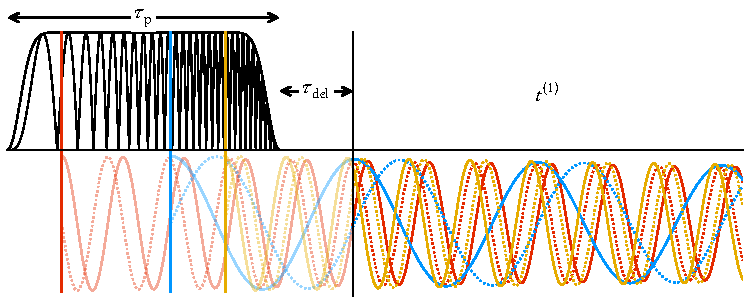
\includegraphics{single_chirp_illustration/single_chirp_illustration.pdf}
    \caption[
        An illustration of an experiment comprising a single chirp pulse.
    ]
    {
        An illustration of an experiment comprising a single chirp pulse sweeping
        low to high frequencies of duration $\tau_{\text{p}}$, followed by
        a pre-scan delay period of time $\tau_{\text{del}}$, prior to
        acquisition. The fate of three resonances with different frequencies is
        denoted, with $f_{\text{red}} < f_{\text{blue}} <
        f_{\text{yellow}}$. Each resonance is excited at different points
        in time, with lower frequency resonances being excited earlier, such that
        each of these evolves for different amounts of time prior
        to acquisition ($\tau_0$).
        The resulting \ac{FID} comprises signals whose phases depend on their
        frequencies quadratically.
        Coloured oscillations denote the evolution of each resonance, with
        solid and dashed lines representing real and imaginary components,
        respectively. It is assumed that the pulse rotates each
        resonance so as to be in phase with the receiver at the point of
        excitation.
    }
    \label{fig:single-chirp}
\end{figure}
Focus is limited here to chirp pulses which sweep from low to high
frequencies; the are parameterised by
their duration $\tau_{\text{p}}$ (\unit{\second}),
excitation bandwidth $\Updelta F$ (\unit{\hertz}),
and \ac{RF} ``amplitude'' $\omega_{\text{RF}}$ (\unit{\hertz}).
The frequencies that a pulse sweeps through are in the range
$[\foff - \nicefrac{1}{2} \Updelta F,
\foff + \nicefrac{1}{2} \Updelta F]$,
and the rate at which the frequency of the chirp is increased (the sweep
rate) is given by $\nicefrac{\Updelta F}{\tau_{\text{p}}}$.
\Cref{fig:single-chirp} provides an illustration of a single chirp
excitation experiment. After application of the chirp pulse, there is typically
a short pre-scan delay $\tau_{\text{del}}$, usually on the order of a few
\unit{\micro\second}, prior to the start of acquisition. While the pre-scan
delay can be determined if an intimate knowledge of the spectrometer hardware
is known, this varies from instrument to instrument, and is not trivial to
ascertain. It is this delay which induces a first-order phase shift in \ac{NMR}
experiments, and which is routinely corrected for by phase correction.
The various chirp pulse parameters are inter-related as
follows\cite{Foroozandeh2019,Kupce1995b}:
\begin{equation}
    \omega_{\text{RF}} = \sqrt{
        \frac{\Updelta F Q}{2 \pi \tau_{\text{p}}}
    },
\end{equation}
where $Q \in \mathbb{R}_{>0}$ is the \emph{adiabaticity factor}.
For a pulse with flip angle  $\beta < \ang{180}$, $Q$ is related to $\beta$ via
\begin{equation}
    Q = \frac{2}{\pi} \ln \left( \frac{2}{\cos(\beta) + 1} \right),
\end{equation}
such that an appropriate pulse to achieve a flip angle of \ang{90} requires
selecting a combination of $\omega_{\text{RF}}$, $\Updelta F$, and
$\tau_{\text{p}}$ which satisfies $Q \approx 0.441$.
The combination used in examples in this work are $\Updelta F =
\qty{400}{\kilo\hertz}$, $\tau_{\text{p}} = \qty{100}{\micro\second}$, and
$\omega_{\text{RF}} \approx \qty{16.8}{\kilo\hertz}$.
For a pulse with sufficiently low $\omega_{\text{RF}}$\,---\,this requires a
sufficiently large pulse duration for a given excitation bandwidth\,---\,it is
reasonable to assume that the chirp pulse induces an instantaneous \ang{90}
rotation at the point of resonance, as depicted in
\cref{fig:single-chirp}. As such, resonances with different
Larmor frequencies evolve for different amounts of time prior to the start of
acquisition, according to
\begin{equation}
    \tau_0\left(f\right) =
        \tau_{\text{del}} + \frac{\tau_{\text{p}}}{2} -
        \frac{(f - \foff) \tau_{\text{p}}}{2 \Updelta F}.
    \label{eq:t0}
\end{equation}
$\tau_{\text{del}} + \nicefrac{\tau_{\text{p}}}{2}$ is the amount of time
between excitation and detection for the on-resonance case, in which
excitation occurs exactly halfway through the pulse. Resonances
with a frequency smaller than that of the transmitter are excited earlier and hence
have a larger $\tau_0$, while the converse is true for resonances with greater
frequencies. The resulting overall phase as of a signal a function of its
frequency can be approximated as\cite{Foroozandeh2019}
\begin{equation}
    \phi(f) = \phi_0 + 2 \pi \left(\tau_{\text{del}} + \frac{\tau_{\text{p}}}{2} \right) (f - \foff) -
        2 \pi \left(\frac{\tau_{\text{p}}}{2 \Updelta F}\right)
        (f - \foff)^2.
    \label{eq:quadratic-phase}
\end{equation}
One might assume that it is possible to generate phased spectra by simply
applying phase correction to the spectrum generated, via
\begin{equation}
    s_{\phi}(f) = s(f) \exp(-\iu \phi(f)).
        \label{eq:spec-phase-chili}
\end{equation}
While the quadratic phase behaviour of peaks is corrected by doing this,
another issue with the dataset is not addressed;
for any resonance, the signal that is detected can be thought of as
the difference between two signals:
\begin{enumerate}
    \item The ``complete'' signal, which starts at the time of excitation.
    \item A ``truncated'' signal which is identical to the complete signal
        before acquisition, and which comprises zeros once acquisition has
        begun.
\end{enumerate}
The linear nature of the \ac{FT} dictates that the
resulting delayed-acquisition spectrum comprises the difference between the
\acp{FT} of the complete signal and the truncated signal.  The \ac{FT} of a
severely
truncated \ac{FID} comprises a broad sinc function with its maximum
at the signal frequency. The appearance of the sinc wiggle depends on
the gap between excitation and acquisition; resonances of lower
frequencies will exhibit deeper, narrower artefacts since the signal is more
significantly truncated. The result of applying quadratic phase correction is
therefore a spectrum of well-phased peaks, but with major baseline distortions,
particularly in the low-frequency region. Figures \ref{fig:bbqchili-sim}.b and
\ref{fig:bbqchili-real}.b both provide examples of this phenomenon.

\subsection{Methodology}
Both the quadratic phase behaviour and delay-induced baseline distortions can
be resolved if an estimate of the \ac{FID}'s parameters is obtained. This enables
the construction of a synthetic \ac{FID} featuring oscillators which are
back-propagated, such that they begin not at the point of acquisition, but at
the point of excitation. The appropriate start time for an oscillator with
frequency $f$ is given by $-\tau_0$, with $\tau_0$ defined in \cref{eq:t0}. The
resulting corrected \ac{FID} $\by \in \mathbb{C}^N$ is defined as
\begin{equation}
    y_n = \sum_{m=1}^{M} \amexpphim \exp((2 \pi \iu (f_m - \foff) - \eta_m) (n \Dt - \tau_0(f_m)))\quad
        \forall n \in \lbrace 0, \cdots, N-1 \rbrace.
    \label{eq:backprop}
\end{equation}
This concept has similarities to the use of \ac{LP} in order to back-propagate
an \ac{FID} to correct for corrupted initial points. However, a holistic
approach such as \ac{LP} cannot be used in this application, as each signal
component must be treated differently according to its frequency.

Thus far in this work, it has been assumed that all signals which make up a
dataset are of the same phase. Of course this isn't the case for \acp{FID}
generated from single-chirp excitation. As such, it is inappropriate to
incorporate the variance of oscillator phases in the fidelity for \ac{NLP}.
For the examples presented in this section, \ac{NLP} was not applied at all;
the direct output of the \ac{MPM} was used as the estimate of the \acp{FID}
parameters.

\subsection{Results}
\begin{figure}
    \centering
    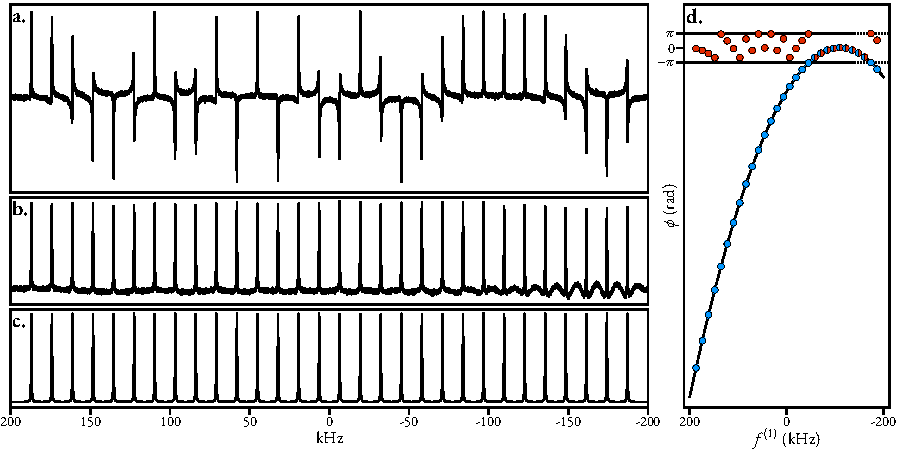
\includegraphics{chirp_phase_vs_estimation/chirp_phase_vs_estimation.pdf}
    \caption[
        A comparison of quadratic phase correction vs frequency-dependent
        back-propagation in treating simulated single-chirp excitation data.
    ]
    {
        A comparison of quadratic phase correction vs frequency-dependent
        back-propagation in treating simulated single-chirp excitation data.
        \textbf{a.} Simulated spectrum for a spin system comprising 30 spins
        with uniformly-separated resonance frequencies. The data was generated
        with
        $N=2^{14}$,
        $\fsw=\qty{400}{\kilo\hertz}$,
        $\foff=\qty{0}{\hertz}$,
        $\tau_{\text{p}} = \qty{100}{\micro\second}$,
        $\tau_{\text{del}} = \qty{0}{\second}$,
        $\Updelta F = \qty{400}{\kilo\hertz}$.
        Coloured lines depict individual oscillators generated using the
        \ac{MPM}; these have been slightly offset for clarity.
        \textbf{b.} Spectrum generated using quadratic phase correction
        (\cref{eq:spec-phase-chili}).
        \textbf{c.} Spectrum generated using the back-propagation approach.
        \textbf{d.} Estimated phases of each oscillator as a function of
        frequency. Red points: phases wrapped within the range $(-\pi, \pi]$.
        Blue points: the same phases, adjusted by addition of a suitable multiple
        of $2 \pi$ to each red point in order to display their quadratic
        dependence on frequency.
        Black curve: quadratic fit of the blue points. The equation of the
        quadratic is stated.
    }
    \label{fig:bbqchili-sim}
\end{figure}
\Cref{fig:bbqchili-sim,fig:bbqchili-real} present comparisons
between the application of quadratic phase correction and the proposed
back-propagation procedure. In the former, a simulated
dataset is considered, comprising 30 evenly-spaced signals, and generated using
\cref{eq:backprop} with $-\tau_0(f_m)$ replaced with $+\tau_0(f_m)$. Other
relevant parameters used are stated in the caption.
A very large damping factor ($\qty{1000}{\per\second}$) was assigned to each
oscillator, as this augments the baseline distortions in the spectrum.
\ac{AWGN} was added to the \ac{FID}, with a target \ac{SNR} of
\qty{25}{\deci\bel}.

The spectrum after quadratic phase correction (\cref{fig:bbqchili-sim}.b)
exhibits the undesired baseline distortions as discussed, with more intense,
narrower baseline distortions associated with lower-frequency signals.
The \ac{MPM} was used to estimate the \ac{FID}'s parameters,
with only the first 2048 points considered
Performing the \ac{MPM} on a signal with $2^{14}$ points would take (a) a
long time, and (b) require a very large amount of \ac{RAM} (see Figures
\ref{fig:mpm-profiling}.a1 and \ref{fig:mpm-profiling}.a2).
Estimating a truncated \ac{FID} comprising the first 2048 points of the
data is justifiable here, since all signal frequencies are spaced
reasonably far apart, meaning each signal in the \ac{FID} becomes
resolvable from the others early on into evolution.
The spectrum generated via back-propagation is presented in
\cref{fig:bbqchili-sim}.c, which is well-phased, and does not suffer from
severe baseline distortion. The variation of the estimated oscillator
phases against their frequencies is plotted in \cref{fig:bbqchili-sim}.d, with
the quadratic dependence clearly illustrated; fitting the blue points to a
quadratic function yielded a second-order coefficient of
$\qty{-7.85e-10}{\radian\second\squared}$, in agreement with the expected value
of $-2 \pi \left(\nicefrac{\tau_{\text{p}}}{2 \Updelta F}\right)$.

\Cref{fig:bbqchili-real} features an experimental dataset, acquired
from a sample of 1\% \ch{Gd}-doped \ch{H2O} in \ch{D2O}\footnote{
    The paramagnetic species \ch{Gd^{III}} is a popular
    contrast agent used in \ac{MRI}, owing to its ability to decrease the $T_1$
    of nearby spins. This typically has an influence on $T_2$ too, with it
    being shortened at high enough concentrations.
    The signal from \ch{H2O} therefore decays at a more rapid rate, such that
    the baseline distortions observed in the phased spectrum of
    \cref{fig:bbqchili-real}.b are more pronounced.
}.
The dataset was acquired using a \ac{2D} experiment, in which the transmitter
offset was adjusted in each increment. The resulting dataset was a series of
\acp{FID}, each comprising a single \ch{H2O} signal with differing frequencies.
When summed, these produce an \ac{FID} with multiple signals at frequencies
defined the selections of transmitter frequencies. The resulting spectrum is
presented in \cref{fig:bbqchili-real}.a.

To produce the phased spectrum in \cref{fig:bbqchili-real}.b, only the
second-order phase was automatically corrected; afterwards, manual
first-order phase correction was applied to the spectrum. This was done
because, as stated above, the
length of the spectrometer delay $\tau_{\text{del}}$ is not trivial to
determine. As with the simulated case, severe baseline distortions exist in the
spectrum, making it unsuitable for quantitative applications.
Analogously, to generate the spectrum via back-propagation, only the
contribution to $\tau_0$ which is dependent on the signal frequency was
included, i.e. $\tau_0$ in \cref{eq:backprop} was replaced with
\begin{equation}
    \tau_{0}^{\prime} = -\frac{(f - \foff) \tau_{\text{p}}}{2 \Delta F}.
\end{equation}
First-order phase correction was then applied to the spectrum produced from the
back-propagated \ac{FID} to yield the result presented in
\cref{fig:bbqchili-real}.c.
In comparison with the quadratic phase-correction approach, it is evident that
a far cleaner spectral baseline is achieved. The phases are not perfectly
consistent across all signals; most notably, the highest- and
second-lowest-frequency signals have phases which stray noticeably from
\ang{0}; it is likely that this resulted from error associated with the
\ac{MPM}. Regardless, it is undeniable that the spectrum produced by
back-propagation achieves a far more desirable result relative to the quadratic
phasing approach.

\begin{figure}
    \centering
    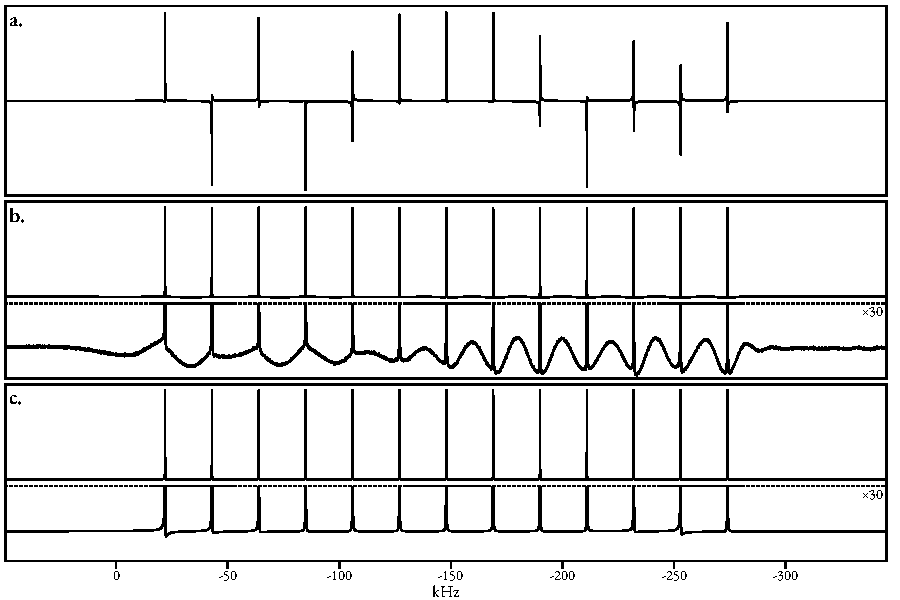
\includegraphics{chirp_phase_vs_estimation_real_data/chirp_phase_vs_estimation_real_data.pdf}
    \caption[
        A comparison of quadratic phase correction vs frequency-dependent
        back-propagation in treating experimental single-chirp excitation data
        generated from a sample of Gd-doped H\textsubscript{2}O in
        D\textsubscript{2}O.
    ]{
        A comparison of quadratic phase correction vs frequency-dependent
        back-propagation in treating experimental single-chirp excitation data
        generated from a sample of 1\% Gd-doped H\textsubscript{2}O in
        D\textsubscript{2}O.
        \textbf{a.} Spectrum generated directly from the acquired \ac{FID}.
        \textbf{b.} Spectrum generated using quadratic phase correction.
        \textbf{c.} Spectrum generated using the back-propagation approach.
    }
    \label{fig:bbqchili-real}
\end{figure}

\section{Summary}

In this chapter, numerous results have been presented, all of which feature
\ac{1D} \ac{FID} estimation.
In \cref{sec:evaluation}, it was illustrated that extending the \ac{MPM}, with
the added step of a phase variance-regularised \ac{NLP} routine, can
aid in the generation of parameter estimates which agree better with the
underlying assumptions of the data structure. Oscillators in the \ac{MPM} often
possess spurious phases; this feature can frequently be rectified by the
\ac{NLP} method. Beyond simply providing a description of the signals which
make up a dataset, it has been shown that parametric estimation can be applied
to further useful ends; two such examples have been presented in
\cref{sec:seq,sec:bbqchili}, respectively.

There are scenarios in which \ac{1D} estimation can perform admirably,
enhancing the information accessible to a spectroscopist. However,
\ac{1D} datasets are typically the most challenging form of \ac{NMR} data to
estimate due to their inherent complexity; with all information about a
sample being distilled into a single dimension, it is very common
(particularly with \ch{^{1}H} datasets) for \acp{FID} to be so densely
populated with signals that extracting meaningful information at
the per-signal level is futile.
\correction{
    It should therefore be appreciated that estimation methods such as the one
    presented in this work\,---\,requiring little to no prior knowledge about
    the dataset to operate\,---\,can only be applied effectively to a limited
    set of cases.
}\label{corr:limited-scope}

Through the separation of signals into more than one detection dimension,
multidimensional experiments can yield datasets which have sufficiently
well-resolved signals for estimation to be applicable to a wider range of
samples. The \ac{2DJ} experiment is such an example, and the estimation of
datasets acquired using it is the focus of the next chapter.

